\documentclass[11pt]{article}
\usepackage[utf8]{inputenc}
\usepackage{amsfonts,epsfig}
\usepackage[hyphens]{url}
\usepackage{hyperref}
\usepackage{breakurl}
\usepackage[authoryear]{natbib}


%%% Document layout, margins
\usepackage{geometry} 
\geometry{letterpaper, textwidth=6.5in, textheight=9in, marginparsep=1em}
%%% Section headings
\usepackage{sectsty} 
\usepackage[normalem]{ulem} 
\sectionfont{\sffamily\bfseries\upshape\large}
\subsectionfont{\sffamily\bfseries\upshape\normalsize} 
\subsubsectionfont{\sffamily\bfseries\upshape\normalsize} 
\makeatletter
%
\usepackage{graphicx}
\usepackage{wrapfig}
 \usepackage{graphicx,fullpage,amsmath,multicol,multirow,amssymb,amsbsy,pifont}
 \usepackage{setspace}
 \usepackage{epsfig}
 \usepackage{amsmath, amsthm, amssymb, bm}
 \usepackage{color}
\usepackage{graphics}
\usepackage{wrapfig}

\newcommand \tcr[1]{\textcolor{red}{(#1)}}
\newcommand \bP{\mathbb{P}}
\newcommand \bE{\mathbb{E}}

\renewcommand\@seccntformat[1]{\csname the#1\endcsname.\quad}



\makeatletter
\def\@maketitle{%
  \begin{center}%
  \let \footnote \thanks
    {\large \@title \par}%
    {\normalsize
      \begin{tabular}[t]{c}%
        \@author
      \end{tabular}\par}%
    {\small \@date}%
  \end{center}%
}
\makeatother



\title{\bf Bayesian hierarchical weighting adjustment and survey inference\footnote{We thank the U.S. National Science Foundation and the Office of Naval Research for grant support.}\vspace{.1in}}
% NSF-MMS Grant SES1534400 and 1534414
\author{Yajuan Si and Andrew Gelman\vspace{.1in}}
\date{5 June 2017}

\begin{document}
\maketitle


\begin{abstract}
We combine Bayesian prediction and weighted inference as a unified approach to survey inference. The general principles of Bayesian analysis imply that models for survey outcomes should be conditional on all variables that affect the probability of inclusion. We incorporate the weighting variables under the framework of multilevel regression and poststratification, and as a byproduct generating model-based weights after smoothing.  We introduce structured prior distributions for smoothing and stability of estimates. We use Stan for computation and in a simulation study compare with classical weightss. We apply the proposal to the New York Longitudinal Survey of Poverty. The new approach increases efficiency for finite population inference, especially for subsets of the population.
\end{abstract}
%%%%%%%%%%%%%%%%%%%%%%%%%%%%%%%%%%%%%%%%%%%
\section{Introduction}

Survey data can be unrepresentative of the underlying population due to planned design features and unplanned nonresponse or undercoverage issues. Arguments between design-based and model-based inference have a long history in survey sampling~\citep{little04-model}. The former automatically takes into account of survey design, while the latter can yield robust inference for small sample estimation. Design-based approaches use weights to balance the sample and the population; see \cite{samsi:review17} for a review of various weighted estimators for a survey population mean. However, classical survey weighting is in practice subject to many user-defined choices such that the process of weighting is difficult to codify \citep{gelman07}. The Bayesian approach for finite population inference~\citep{ghosh:meeden:97} allows prior information to be incorporated, when appropriate, but is subject to model misspecification.

In the present paper we combine Bayesian prediction and weighted inference as a unified approach to survey inference, applying robust Bayesian regression models to account for complex design features under the framework of multilevel regression and poststratification (MRP, \cite{gelman:little:97,park:gelman:bafumi-04,Ghitza:gelman-13}). The proposal yields design-consistent and efficient finite population inference and constructs model-based weights after smoothing.

For a finite population of $N$ units, we denote the variable of interest as $y=(y_1,\dots,y_N)$ and the inclusion indicator variable as $I=(I_1,\dots,I_N)$, where $I_i=1$ if unit $i$ is included in the sample and $I_i=0$ otherwise. Here, inclusion refers to selection and response. Design-based inference considers the distribution of $I$ and treats $y$ as fixed. Model-based inference considers the joint distribution for $I$ and $y$.

To account for the factors that affect inclusion, design weights adjust for unequal probabilities of sampling, and the subsequent weighting accounts for coverage problems and nonresponse during data collection or data cleaning. Classical weights are thus generated as a product of multiple adjustment factors: inverse probability of selection, inverse propensity score of response, and poststratification~\citep{hs79} (also called calibration, benchmarking) ratios.  Each of these adjustments can be approximate when probability of selection, probability of response, or population totals are estimated from data.  Beyond any approximation issues, even if the inclusion model is known exactly, extreme values of weights will cause high variability and then inferential problems, especially when the weights are weakly correlated with the survey outcome variable. When the weighting process involves poststratification or nonresponse adjustment---where the weights themselves are random variables---the variance estimation will be different from the cases only with fixed design weights. It is non-trivial to derive a variance estimator under multi-stage weighting adjustment or complex sampling design.

In practice, the construction of survey weights requires somewhat arbitrary decisions of the selection of variables and interactions, pooling of weighting cells, and weight trimming. It is unclear whether and how to incorporate auxiliary information~\citep{groves:couper:98JOS}.  Discussion of smoothing and trimming in the survey weighting literature \cite[e.g.][]{potter88,trim-potter90,modeltrim-elliottandlittle00,elliott07,elliot:JOS16} has focused on estimating the finite population total or mean, with less attention to  subdomain estimates. \cite{beaumont08} proposes to smooth weights by predicting and regressing these on the survey variables. Borrowing information on survey outcomes potentially increases efficiency and calls for a general framework.

Under probability sampling, model-based inferences can be based on the distribution of $y$ alone given the weighting variables are included in the model~\citep{rubin76,rubin83-pi}. The inclusion mechanism is ignorable when the distribution of $I$ given $y$ is independent of the distribution of $y$ conditional on the weighting variables. \cite{gelman07} recommends regression models including weighting variables as covariates.  Any of these approaches can be sensitive to prior specification for stable estimation; this is the model-based counterpart to the decisions required for smoothing or trimming classical survey weights.

Model-based and model-assisted weighting adjustment methods for finite population total estimation have been compared by  \cite{henry:valliant12}. The model-based weighting methods in the superpopulation perspective~\citep{FPSi:Valliant00} use predictions from regression models to derive case weights, where the predictions are based on hierarchical linear regression models with various bias corrections~\citep{robustblup:Chambers:JASA93,robust:Firth:JRSSB98}. The model-assisted methods derive case weights mainly from calibration on benchmark variables~\citep{calibration:kott09} via the generalized regression estimator (GREG,~\cite{greg92}) and penalized spline regression estimators~\citep{breidt05}. However, the case weights derived from regression predictions can be highly variable and even negative, and may damage some domain estimates.
To protect against model misspecification, \cite{little83-pi} recommends modeling differences in the distribution of outcomes across classes defined by differential probabilities of inclusion. \cite{bnfp:ba15} construct poststratification cells based on the unique values of inclusion probabilities and build hierarchical models to smooth cell estimates as advocated by \cite{little91, little93}. 


We propose to use Bayesian hierarchical models accounting for survey design to generate weights that can be used in design-based inference. For large samples, the inference will parallel with design-based inference. For small samples, the hierarchical model smoothing will stabilize domain estimation and generate robust weighting adjustment.

We use the intrinsic weighting variables, assume they are discretized and construct poststratification cells based on the cross-tabulation. Weights are derived through the regressing survey outcome on weighting variables given the poststratification. The inclusion of the outcome variable into weighting and poststratification both avoid model misspecification and potentially increase efficiency~\citep{fuller09}. Multilevel model estimates shrink the cell estimates towards the prediction from the regression model. The MRP framework combines multilevel regression and poststratification, accounts for design features in the Bayesian paradigm, and is then well equipped to handle complex design features.

\cite{bnfp:ba15} incorporate weights into MRP, increasing efficiency comparing to the pseudo-likelihood approach~\citep{pfeffermann93}. In the present paper we go further, starting from the variables that are used for weighting and constructing model-based weights as byproducts under MRP. We develop a novel prior specification for the regularization to handle potentially large numbers of poststratification cells. The prior setting allows for variable selection and keeps the hierarchical structure among main effects and high-order interaction terms for categorical variables. That is, if one variable is not predictive, then the high-order interactions involved with this variable are also likely to be not predictive, to facilitate model interpretation.

We implement the posterior computation via Stan~\citep{stan-software:2013,stan-manual:2013}, which uses Hamiltonian Monte Carlo sampler with adaptive path lengths~\citep{hoffman-gelman:2012}.  Stan promotes robust model-based approaches by reducing the computational burden of building and testing new models. Stan provides the accessible platform and has the potential to support the unified framework for survey inference.

Section~\ref{problem} introduced the motivating problem to construct weights for an ongoing social science survey. We discuss the detail of our proposed method in Section~\ref{method}. Section~\ref{simulation} describes the statistical evaluation on model-based prediction and weighting inference, and comparison with classical weighting. We apply the proposal to the reallife survey in Section~\ref{application} and demonstrate the efficiency agains. Section~\ref{discussion} summarizes the improvement and discusses further extension.

%%%%%%%%%%%%%%%%%%%%%%%%%%%%%%%%%%%%%%%%%%%
\section{The motivating application}
\label{problem}
	
Our methodological research is motivated by operational weighting practice for ongoing surveys. Our immediate goal is to construct weights for the New York City Longitudinal Study of Wellbeing  (LSW) \citep{RHweighting,RHreport}, a survey organized by the Columbia University Population Research Center, aiming to provide assessments of income poverty, material hardship, and child and family wellbeing of NYC residents.

We use the LSW as an example to illustrate practical weighting issues and our proposed improvement, with the understanding that similar concerns arise in other other surveys. The sample includes a phone sample based on random digit dialing and an in-person respondent driven sample of beneficiaries from Robin Hood philanthropic services and their acquaintances. We focus on the phone survey here as an illustration. The LSW phone survey interviews 2,002 NYC adult residents, including 500 cell phone calls and 1502 landline telephone calls, where half of the landline samples are from low-income NYC areas defined by zipcode information. The collected baseline samples are followed up every three months. We match the samples to the 2011 American Community Survey (ACS) records for New York City. The discrepancies are mainly caused by the oversampling of the low-income neighborhoods and nonresponse. 

The baseline weighting process~\citep{RHweighting} adjusts for the unequal probability of selection, coverage bias, and nonresponse. Classical weights are products of estimated inverse probability of inclusion and raking~\citep{gr-rake93} ratios. However, practitioners have to make arbitrary or subjective choices on the selection and values of weighting factors. For example, to construct weights for individual adults, we have to weight up respondents from large households, as just one adult per sampled household is included in the sample. \cite{gelman:little:98} recommend the square root of the ratio of household sizes to family sizes for this weighting adjustment because using household sizes as weights~\cite[for example,][]{acsweighting2014} tend to overcorrect in telephone surveys. In practice the raking procedure adjusts for socio-demographic factors without tailoring for particular surveys.
	
The survey organizers are interested in the aspects of quality of life of city residents, such as the percentage of children who live under poverty and material hardship. Thus it is important to get accurate estimates for subpopulations. We would like to develop an objective procedure and let the collected survey data determine the weighting process. The basic principle is to adjust for all variables that could affect the selection and response into weighting. Ideally, we expect that weighting variables should include phone availability (number of landline/cell phones and duration with interrupted service), family size, household size, and socio-demographics. However, the ACS records only provide information on family size, age, ethnicity, sex, education and poverty gap (a family poverty measure). Meanwhile, considering the substantive analysis goal, the variables describing the number of elder people in the family, the number of children in the family, and the family size, as well as their interactions with poverty gap are recommended by the survey organizers to be included into the weighting process to balance the distribution discrepancy with the population. 
	
To generate classical weights, we select the raking factors that could affect the selection and response, including sex, age, education, ethnicity, poverty gap, the number of children in the family, the number of elder people in the family, the number of working aged people in the family, the two-way interaction between age and poverty gap, the two-way interaction between the number of persons in the family and poverty gap, the two-way interaction between the number of children in the family and poverty gap, and the two-way interaction between the number of elder people in the family and poverty gap. We collect the marginal distributions from ACS and implement raking adjustment. 
		
However, it is possible that the subjective weighting adjustment includes some variables or interactions that are not essentially predictive or does not take account for all the important factors that could be of substantive interest later. The raking adjustment assumes that these factors are independent. This will cause biased domain inference if the correlation structure in the sample is different from that in the population. Ideally, we should match based on the joint distribution of these weighting related variables. However, small cell sizes or empty under the deep interactions will lead to extremely large weights that need cell collapsing. 
	
	The problems about classical weighting faced by the LSW baseline are general enough that they occur for most operational weighting practice in real-life surveys, which could be complicated with complex design, longitudinal structure or multi-stage response mechanisms. Usually different weighting practitioners generate different weights and then weighted analyses, causing weighted inference a mess. It is important to propose a model-based weighting procedure that allows the data to select weighting factors without arbitrary choices and facilitates domain estimates. We would like to incorporate these weighting variables into the model for survey outcomes for efficiency gains, model their high-order interaction terms under regularized prior setting and generate the weights that can be equally treated as classical weights. Large number of weighting variables and deep interactions will cause small weighting cells based on the cross-tabulation. The small weighting cells call for statistical adjustment for smoothness and stability. 
		
	MRP have achieved success for domain estimation at much finer levels. Borrowing the strength of hierarchical modeling framework with informative prior distribution, we should be able to obtain the estimate after smoothing the sparse cells. Poststratification via census information will match the estimate from the sample to the population. The combination of regression and poststratification is similar with the endogenous poststratification concept~\citep{Breidt08,Dahlke13}. We introduce the MRP framework in detail.
	

	
%%%%%%%%%%%%%%%%%%%%%%%%%%%%%%%%%%%%%%%%%%%
\section{Method}
\label{method}

\subsection{Multilevel regression and poststratification}
In the basic setting, we are interested in estimating the population distribution of the survey outcome $y$. When the weighting process is transparent, we can directly include the weighting variable $X$ into regression modeling for the survey outcome $y$. Here $X$ is a $q$-dimensional vector of variables that affect the sampling design, nonresponse and poststratification. Conditional on $X$, the distribution of inclusion indicator $I$ is ignorable. Under MRP, the weighting variables $X$ are discretized, and their cross-tabulation constructs the poststratification cells $j$, with population cell sizes $N_j$ and sample cell sizes $n_j$. Then the total population size is $N=\sum_{j=1}^J N_j$, and the sample size is $n=\sum_{j=1}^Jn_j$, where $J$ is the total number of poststratification cells \citep{little91, little93, gelman:little-97,gelmancarlin01}. 

Post-stratification inference is different from design-base inference under stratified sampling by the fact that $n_j$'s are now random functions of the sampling distribution $I$. In repeated sampling of $I$, there is a non-zero probability that $n_j=0$ for some $j$. The usual resolution of this problem is to condition on $n_j$'s observed in the realized sample, however, the sample inference is not design-unbiased conditionally on $n_j$'s. The MRP framework assumes a model for $n_j$'s and preserves design consistency.
	
The poststratification implicitly assumes that the units in each cell are included with equal probability. Suppose $\theta$ is the population estimand of interest, such as the overall or domain mean, and it can be expressed as a weighted sum over any subset or domain $D$ of the poststrata,
\begin{align}
	\theta=\frac{\sum_{j\in D}N_j\theta_j}{\sum_{j\in D}N_j},
\end{align}
where $\theta_j$ is the corresponding estimand in cell $j$. 
The proposed poststratified estimator will be of the general form,
\begin{align}
\label{model-based}
	\tilde{\theta}^{\textrm{PS}}=\frac{\sum_{j\in D}N_j\tilde{\theta_j}}{\sum_{j\in D}N_j},
\end{align}
where $\tilde{\theta}_j$ is the corresponding estimate in cell $j$. Various modeling approaches can be used to estimate the cell estimates, such as the flexible nonparametric Bayesian models and machine learning algorithms. Here, we illustrate using a hierarchical regression model.

In practice, survey weights are attached to each unit, even though they are not attributes of individual units. It is natural to generate unit-level weights based on the entire survey design, and use the weighted averages of the form, such as $\tilde{\theta}=\sum_{i=1}^n w_i y_i/\sum_{i=1}^nw_i$. Our goal here is to obtain an equivalent set of unit-level weights $w_i$ through a model-based procedure for the estimation of $\tilde{\theta}^{\textrm{PS}}$ to connect weighting and poststratification. Therefore, regression models can be used to obtain $\tilde{\theta}_j$, poststratification accounts for the population information, and model-based weights are re-derived via expression (\ref{model-based}).
	
In classical regression models, full poststratification is a special case, where the cell estimates are computed separately for each cell without any pooling effect. For example, if we are interested in the population mean, then the cell means will be used as the cell estimates. Generally, classical regression models are conducted on cell characteristics without going to the extreme fitting separately for each cell. If more interactions among the characteristics are included, the resulted weights become more variable. On the other side, complete pooling ignores the heterogeneity among cells. Hierarchical regression models will smooth the variable estimates under partial pooling. 
	
\cite{gelman07} uses the exchangeable normal model as an illustration and shows that the poststratification estimate $\tilde{\theta}^{\textrm{PS}}$ for population mean can be expressed as a weighted average between the cell means and the global mean, which yields the unit weights, also as a weighted average between the completely smoothed weights, $w_j$ = 1, and the weights from full poststratification, $w_j = \frac{N_j/N}{n_j /n}$. Hierarchical poststratification is approximately equivalent to shrinkage of weights through the shrinkage of the parameter estimates. The degree of shrinkage goes to zero as the sample increases, which implies that estimates from the model are design-consistent. However, improvements are necessary to handle large number of cells and deep interactions and evaluate the performance of model-based weights. 

In our application of the Longitudinal Study of Wellbeing, the weighting variables include age (5 categories), ethnicity (5 categories), education (4 categories), sex (2 categories), poverty gap (5 categories), family size (4 categories), number of elder people (3 categories) and number of children (4 categories), in the family, and this results in $J=5\times5\times4\times2\times5\times3\times4\times4=48,000$ poststrata. The majority of the poststratification cells will be empty or sparse due to limited sample size (2,002). The sample cell sizes are unbalanced. Often cells are arbitrarily collapsed or combined~\citep{little93} without theoretical justification. Recent model-based weighting smoothing procedures across cells could not handle such sparse cases~\citep{modeltrim-elliottandlittle00}. \cite{elliot:JOS16} introduce a Laplace prior for weight smoothing across a modest number of poststrata based on inclusion probabilities but ignore the weighting variable hierarchy structure. Using the MRP framework, we  account for the variable hierarchy structure to smooth and pool the estimates across the sparse and unbalanced cell sizes.

\subsection{Structured prior distribution}

We introduce a structured prior distribution to improve MRP under the sparse and unbalanced cell structures, thus yielding stable model-based survey weights that account for design information. For now, suppose the population distribution of $X$ is known, that is, we can obtain $N_j$'s from the external data to describe a joint distribution of the weighting variables. However, the number of poststratification cells $J$ can be large, even much larger than the sample size $n$. Deep interactions are essential for complex relationship structure, but we cannot include all and have to select the predictive main effects and interactions. 

Suppose the collected survey response is continuous, $y_i$, for $i=1,\dots, n$, and we are interested in the population mean $\bar{y}$ estimation. We use $X^{pop}=(X^1,\dots, X^J)^\top$ to represent the $J\times q$ predictor matrix in the population under the poststratification framework. For illustration, assume a normal distribution,
\begin{align}
\label{normal}
	y_i \sim \textrm{N}(\theta_{j[i]}, \sigma_y^2),
\end{align}
where $j[i]$ denotes the cell $j$ that unit $i$ belongs to. We can also consider unequal variances, allowing the cell scale $\sigma_y$ to vary across cells, indexed as $\sigma_j$. For the prior specification of $\theta_j$, one choice can be  $\theta_j=X^j\beta$, and $\beta$ is assigned with hyperprior distribution $\pi(\cdot)$. In the hierarchical regression example of \cite{gelman07}, a multivariate normaldistribution is considered, $y\sim \textrm{N}(X\beta, \Sigma_{y})$ and $\beta \sim \textrm{N}(0,\Sigma_{\beta})$, where the covariates include all main effects and a few selected two-way interactions in $X$ and the covariance matrix $\Sigma_{\beta}$ is diagonal with different scales. However, the model is subject to misspecification, and the generated weights could be negative.
	
Since $X^j$ consists different level indicators of the $q$ discrete weighting variables, we can express the population cell mean $\theta_j$ as
\begin{align}
\label{regression}
	\theta_j=\alpha_0 + \sum_{k\in S^{(1)}}\alpha_{j,k}^{(1)}+\sum_{k\in S^{(2)}}\alpha_{j,k}^{(2)}+\dots+\sum_{k\in S^{(q)}}\alpha_{j,k}^{(q)},
\end{align}
where $S^{(l)}$ is the set of all possible $l$-way interaction terms, and $\alpha^{(l)}_{j,k}$ represents the $k$th of the $l$-way interaction terms in the set $S^{(l)}$ for cell $j$. For example, $\alpha^{(1)}_{j,k}$'s with $k\in S^{(1)}$ refer to the main effects, $\alpha^{(2)}_{j,k}$'s with $k\in S^{(2)}$ being the two-way interaction terms, for cell $j$. This decomposition covers all possible interactions among the $q$ weighting variables. When the cell structure is sparse, variable selection is necessary. In practice, we recommend the initial inclusion of covariates and interactions with substantive importance in Model (\ref{regression}) and perform Bayesian variable selection under the proposed structure prior setting.

We induce structure prior distributions to be able to handle deep interactions and account for their hierarchy structure, where the high-order interaction terms will be excluded if one of the corresponding main effects is not selected. Larger main effects often lead to larger effects of the involved interaction terms. Ideally, more shrinkage should be put on the high-order interactions than that on the main effects, and the prior setting should reflect the nested structure. The challenge embodies the problem in Bayesian inference for group-level variance parameters in an Anova structure~\citep{anova:gelman:05, gelman06-prior}. \cite{volfovsky:hoff14} introduce a class of hierarchical prior distributions for interaction arrays that can adapt to potential similarity between adjacent levels, where the covariance matrix for the high-order interactions is assumed as a Kronecker product of the covariance matrices of main effects after adjusting relative magnitudes. Our proposal extends with a novel set of prior distributions by inducing more structure among the variance parameters, more shrinkage and smoothing effect to handle extremely large number of cells with unbalanced sizes than the generally balanced setting in~\cite{volfovsky:hoff14}. 

We start with independent prior distributions on the regression parameters $\alpha$:
\[\alpha_{j,k}^{(l)}\sim \textrm{N}(0, \lambda_k^{(l)}\sigma^2),\]
where $\lambda_k^{(l)}$ represents the local scale and $\sigma$ is the global error scale, for $k\in S^{(l)}$ and $l=1,\dots, q$. The error scale is the same across the main effects and high-order interactions, while the local scales are different. The shrinkage effect is induced through the specification of local scales. We assume the local scale of high-order interactions is the product of those for the corresponding main effects after adjusting relative magnitudes.
\[\lambda^{(l)}_k=\delta^{(l)}\prod_{l_0\in M^{(k)}}\lambda^{(1)}_{l_0},\]
where $\delta^{(l)}$ is the relative magnitude adjustment and $M^{(k)}$ is the collection of corresponding main effects that construct the $k$th $l$-way interaction in the set $S^{(l)}$. For example, the local scale of the three-way interaction among age, sex, and education, middle-aged men with college education, will be the product of those for the main effects on age, sex, and education, that is, the product of the local scale parameters for middle aged, men, and college educated, respectively. 

We use the following hyperpriors on the scale parameters:
\begin{align}
\label{main}
	\nonumber  \mbox{error scale: }&\sigma \sim  \textrm{Cauchy}_{+}(0,1) \\ 
	\nonumber \mbox{local scale for main effects: } & \lambda_k^{(1)} \sim  \textrm{N}_{+}(0,1)\\
	 \mbox{local scale for high-order interactions: } & \lambda^{(l)}_k=\delta^{(l)}\prod_{l_0\in M^{(k)}}\lambda^{(1)}_{l_0} \\
	\nonumber  \mbox{relative magnitude for high-order interactions: }&\delta^{(l)}  \sim   \textrm{N}_{+}(0,1) \mbox{, for } l=2,\dots, q.
\end{align}
Here $\textrm{Cauchy}_{+}$ and $\textrm{N}_{+}$ denotes the positive part of the Cauchy and normal distributions, respectively.
\cite{gelman06-prior} proposes the half-Cauchy prior for the scale parameter in hierarchical models, which has the appealing property that it allows scale values arbitrarily close to 0, with heavy tails allowing large values when supported by the data. When $\lambda_k^{(l)}$ is close to 0, the posterior samples of $\alpha_{j,k}^{(l)}$ are shrunk towards 0. The scale parameter for the high-order interaction terms will be 0 if any of the related scale parameters for the main effects is 0. The overall regularization effect is determined by the error scale and the multiplicative scale parameters of the corresponding main effects. We assign a noninformative prior distribution to the intercept term and weakly informative prior distributions to the two global error scale parameters $(\sigma_y, \sigma)$.


Our proposed prior specification features the group selection of all possible level indicators for the same variable, similar to the group lasso~\citep{grouplasso06}. We achieve the goal of variable selection under the similar specification with the horseshoe prior distribution~\citep{horseshoe10} and improve by setting group selection and multiplicative scales for high-order interactions for sparsity gains. We introduce weakly informative half-Cauchy prior distributions to error scales and informative half-normal prior distributions to the local scale parameters, in the same spirit as in~\cite{hyperprior:Aki16}, to improve parameter shrinkage estimation and computation efficiency. When the posterior estimation of the scale parameter is close to 0, indicating the variable is not predictive; post-processing can be done to exclude the variable from poststratification cell construction for dimension reduction. This class of priors allows for variable selection in high dimension and keeps the hierarchy structure among main effects and interactions.
 
\subsection{Model-based weights}

We can re-express the model~(\ref{regression}) and~(\ref{main}) as the exchangeable normal model:	
\begin{align}
\label{theta-summary}
	\theta_j \sim N(\alpha_0, \sigma^2_{\theta})\mbox{, } \ \ \sigma^2_{\theta}=\sum_{l=1}^q\sum_{k\in S^{(l)}}(\lambda_k^{(l)}\sigma)^2.
\end{align}
Conditional on the variance parameters, the posterior mean in the normal model with normal prior distribution is a linear function of data; thus we can determine {\em equivalent weights} $w^*_i$'s so that one can re-express the smoothed estimate $\sum_{j=1}^J\frac{N_j}{N}\tilde{\theta}_j$ as a classical weighted average, $\sum_{i=1}^n w^*_iy_i/\sum_{i=1}^n w^*_i$. Combining the posterior mean estimates for $\theta_j$ and the model-based estimate given in (\ref{model-based}), \cite{gelman07} derives the equivalent unit weights in cell $j$ that can be used classically. 
\begin{align}
\label{model-w}
 	w_j\approx \frac{n_j/\sigma^2_y}{n_j/\sigma^2_y+1/\sigma_{\theta}^2}\cdot\frac{N_j/N}{n_j/n} +  \frac{1/\sigma^2_{\theta}}{n_j/	\sigma^2_y+1/\sigma_{\theta}^2} \cdot 1,
\end{align}
where the model-based weight is a weighted average between full poststratification weight without pooling (equal to $\frac{N_j/N}{n_j/n}$) and completely smoothing weight (equal to 1). The shrinkage effect is quantified as $\frac{1}{n_j\sigma^2_{\theta}/	\sigma^2_y	+1}$, where depends on the group and individual scales, as well as sample cell sizes. The model-based weights are random variables, and fully Bayesian inference will capture the corresponding variability. We collect the posterior mean values and treat as the weights that can be used the same as classical weights.

The fully Bayesian inference is realized via Stan. As open source and user friendly software, Stan contributes to the wide application of Bayesian modeling. Survey practitioners resist model-based approaches mainly due to computation burden. However, model-based methods are ready to face the new challenges on big survey data, such as unbalanced cell structure, combining multiple surveys and analyzing streaming data. The development of Stan can improve the generalization of model-based approach and provide the computational platform for the unified survey inference framework.

In our implementation, the Markov chain Monte Carlo samples mix well and the chains converge quickly. The proposed prior specification improves the stability for smoothed weights under partial pooling. To illustrate the capability of variable selection and hierarchy maintenance and the resulting efficiency gains, we compare the posterior estimation with that under independent prior setting but without the multiplicative scale constraint, which is similar with Horseshoe prior under group specification. We  compare the model-based weights with classical weights in Section~\ref{simulation} and~\ref{application} to demonstrate the calibration for design-based properties. Furthermore, we illustrate the proposed improvement for domain estimation under unbalanced and sparse sample cell structure. 


%%%%%%%%%%%%%%%%%%%%%%%%%%%%%%%%%%%%%%%%%%%%%
\section{Simulation studies}
\label{simulation}

We consider two main simulation scenarios: slightly unbalanced structure with a moderate number of poststratification cells and very unbalanced structure with a large number of poststratification cells. We evaluate the statistical validity of the model-based and weighted estimation for the finite population and domain inference to demonstrate the improved capability to solve the classical weighting problems. We consider model-based predictions under the structure prior (Str-P) and the independent prior (Ind-P) distributions. For weighted inference, we evaluate the estimation after applying the model-based weights under structure prior (Str-W) setting, model-based weights under independent prior (Ind-W) distributions, weights obtained via raking adjustment (Rake-W), classical poststratification weights (PS-W), and inverse probability of selection weighting (IP-W). We present the graphical diagnosis tools to compare the weights and weighted inference.

We borrow 2011 ACS survey of NYC adult residents treating it as the ``population", and randomly draw samples out of it according to a prespecified selection model without nonresponse. We collect covariates from ACS and simulate the outcome variable to obtain the true distribution as a benchmark. We implement the raking procedure by balancing the marginal distributions of the weighting variables in the selection model and generate the raking weights. The classical poststratification weights $N_j/n_j$'s are obtained by matching the selected sample cell indices with those of the population cells. The selection model can provide the inverse-probability of selection weights by matching the sampled unit indices. We also generate model-based weights under independent prior distributions for the main effects and high-order interaction terms. The generated weights are normalized to average 1 for comparison convenience. 




%%%%%%%%%%%%%%%%%%%%%%%%%%%%%%%%%%%%%%%%%%%%%%%%%
\subsection{Slightly unbalanced structure}
\label{3var}
We first handle slightly unbalanced structure when the number of poststratification cells and the sample cell sizes are moderate. We implement repeated sampling process to investigate the frequentist properties of model-based predictions and weighted inferences. With little shrinkage effect on high-order interactions, the model-based prediction and weighting with structure prior distributions have similar performance with that under independent prior distributions, while outperforming the classical weighting approaches. 

Assume three weighting variables are included in the selection and outcome models: age, ethnicity, and education. We discretize the three variables in ACS as {\em age} (18--34, 35--44, 45--54, 55--64, 65+), {\em eth} (non-Hispanic white, non-Hispanic black, Asian, Hispanic, other), and {\em edu} (less than high school, high school, some college, bachelor degree or above). The number of poststratification cells is $5\times 5 \times 4 = 100$. 

We assume the outcome depends on deep interactions, including all the main effects, two-way and three-way interaction terms among the three weighting variables; and the selection indicator depends on the three main effects. The specific values of the coefficients are given in Tables~\ref{s1-response-coef}--\ref{s1-selection-coef} in Appendix~\ref{appendix}. The values are set to reflect the strong correlations between the covariate and dependent variables. And the effects are not necessarily similar across the adjacent factor levels, different from the scenarios in~\cite{volfovsky:hoff14}. The error scale in the outcome model is set as 1. 

We repeat the sampling for 200 times. The sample sizes vary between 2141 and 2393 with median 2288. Empty sample cells occur with spread-out selection probabilities (ranging from 0.001 to 0.269) over the repeated sampling process. The number of occupied cells in the sample is between 80 and 93 with median 87. The slightly unbalanced cell structure is common in practice with simple and clean sampling design.
The population quantities of interest include the overall mean, domain means across the $13\, (=5+4+4)$ marginal levels of three weighting variables and domain mean for non-white youths (an example of interaction between age and ethnicity). We examine the absolute value of estimation bias, root mean squared error (RMSE), standard error (SE) approximated by the average value of standard deviations (Ave.\ SD) and nominal coverage rate of the 95\% intervals.



\begin{figure}
\centering
\begin{tabular}{cc}
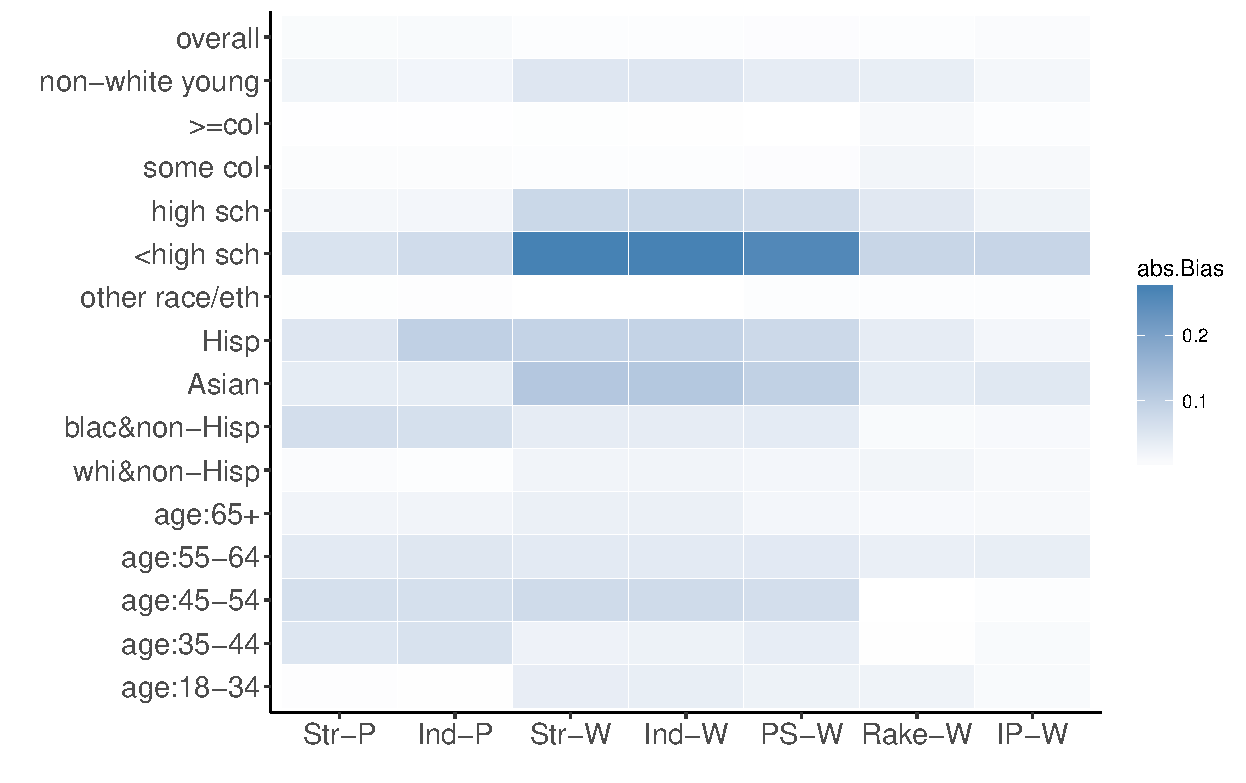
\includegraphics[width=.475\textwidth]{plot/var3_bias_case1.pdf}&
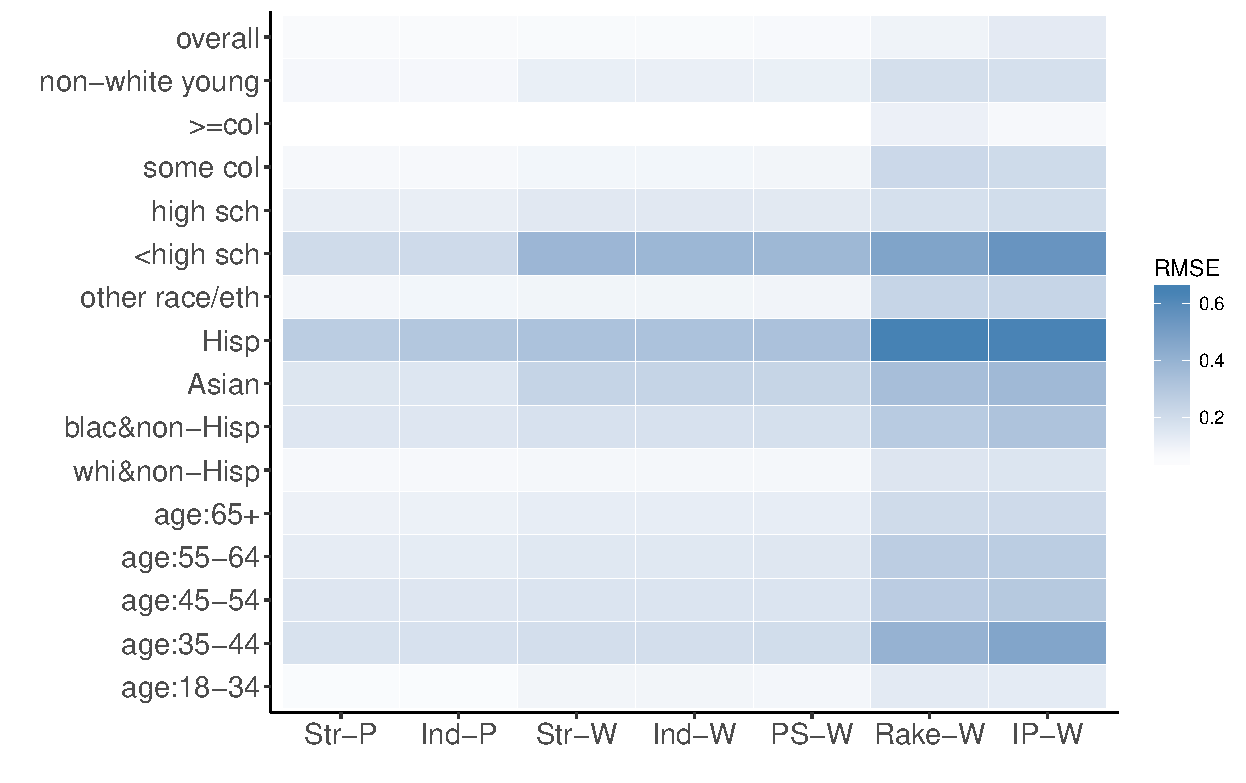
\includegraphics[width=.475\textwidth]{plot/var3_rmse_case1.pdf}\\
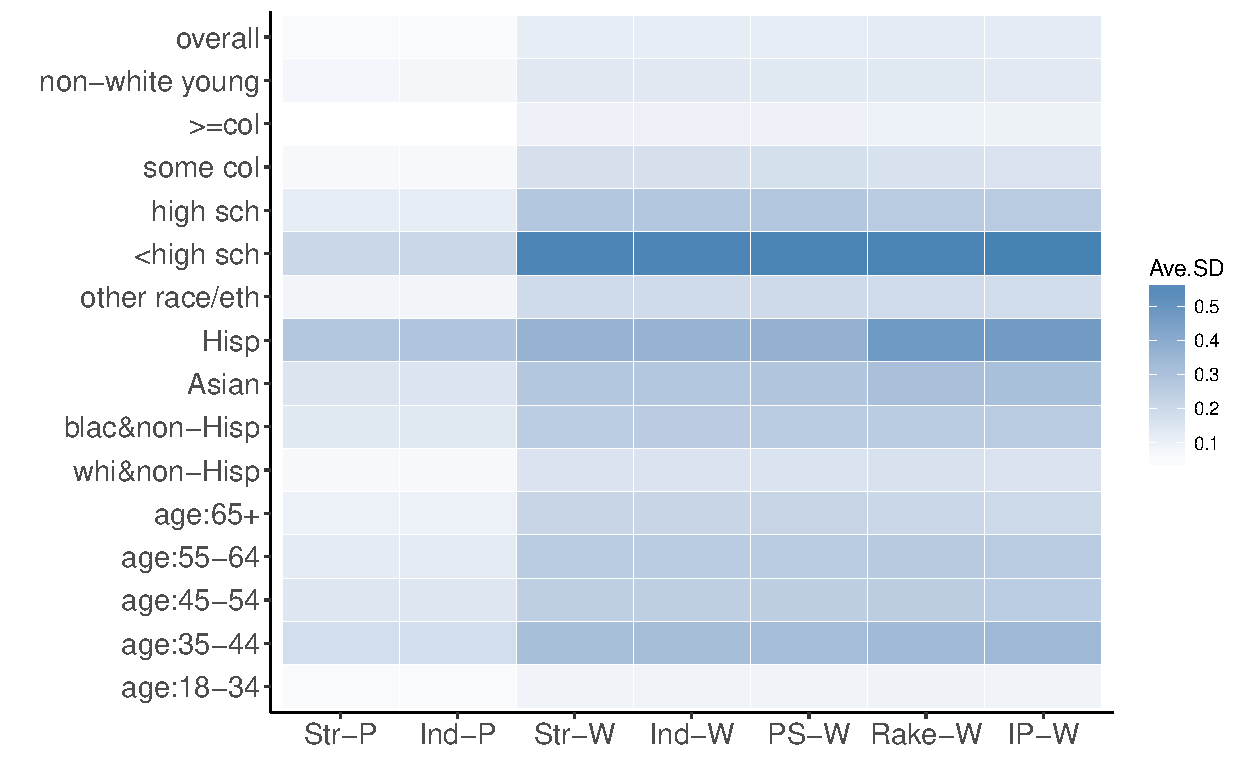
\includegraphics[width=.475\textwidth]{plot/var3_se_case1.pdf}&
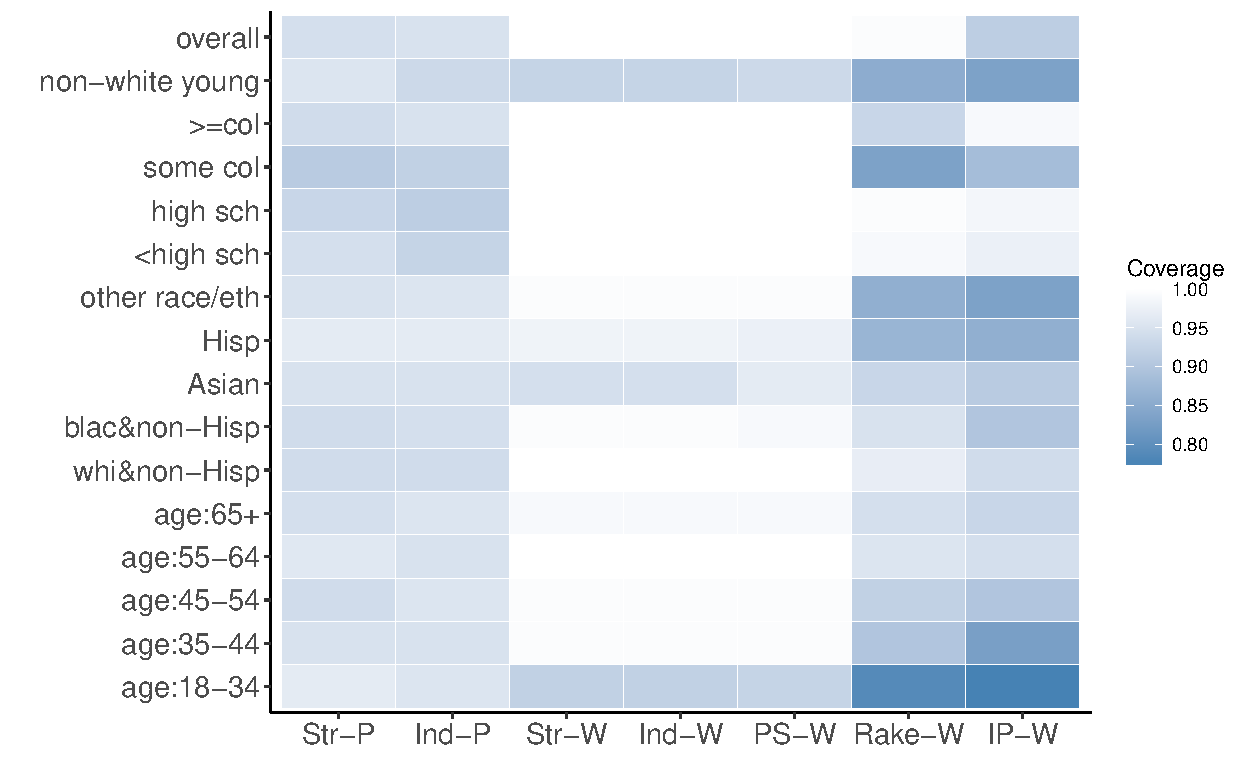
\includegraphics[width=.475\textwidth]{plot/var3_cr_case1.pdf}\\
\end{tabular}
\caption{\em Comparison of prediction and weighting performances on validity of finite population inference under slightly unbalanced design. The y-axis denotes different groups for the mean estimation. The x-axis includes two model-based prediction methods (Str-P, Ind-P), two model-based weighting (Str-W, Ind-W), and three classical weighting methods (PS-W, Rake-W, IP-W). Str-P: model-based prediction under the structure prior; Ind-P: model-based prediction under the independent prior distribution; Str-W: model-based weighting under structure prior; Ind-W: model-based weighting under independent prior distribution; Rake-W: weighting via raking adjustment; PS-W: poststratification weighting; and IP-W: inverse probability of selection weighting. The plots show that the model-based predictions outperform weighting with the smallest RMSE, the smallest SEs, reasonable coverage rates, and comparable bias among all the methods. Model-based weighting inference has smaller RMSE and SEs but more reasonable coverage rates than that with classical weighting.}
\label{sim1}
\end{figure}

The outputs in Figure~\ref{sim1} show that the model predictions have the smallest RMSE, the smallest SEs with reasonable coverage rates, and comparable bias among all the methods. All variables affecting the outcome and selection mechanism are included in the modeling to satisfy the Bayesian principle for ignorable sampling mechanism. The model will predict all the cell estimates including the empty cells in the sample, fully using the population information and poststratification cell structure. The weighting inference is conditional on the observed units within occupied cells, and thus less efficient than the model predictions. Generally, the model-based weighting inference has smaller RMSE and SEs but more reasonable coverage rates than that with classical weighting. Raking adjustment is not valid for the domain estimation with large bias, large RMSE and poor coverage, even though the selection mechanism depends on only the main effects. The inverse probability of selection weighting inference tends to have large SEs but low coverage rates, especially for domain estimation. The poststratification weighting inference is close to the model-based weighting estimation since the domain sizes are modestly large. The cell shrinkage effect towards no weighting is small (between 0 and 0.19 with mean 0.05) under slightly unbalanced design. The number of cases who are less than high school educated is small (around 80), resulting in large estimation bias and SEs for the weighting inferences, but not in model-based predictions. The model-based predictions stabilize the small area estimation by smoothing.

Model prediction performs well and similarly under the structure prior distribution or independent prior distribution. This is expected due to the small shrinkage effect. The cell structure is slightly unbalanced, and the outcome and selection models depend on all the main effects and high-order interaction terms. But the structure prior setting yields more efficient inference than the independent prior setting with small SEs. This improvement is obvious in the very unbalanced design as shown in the following simulation of Section~\ref{8var}.

Additionally, we considered nine cases with different survey outcome models and sample selection models depending on various predictors as in Table~\ref{s1-design} in Appendix~\ref{appendix}. The specific values of the coefficients are given in Tables~\ref{s1-response-coef}--\ref{s1-selection-coef}.The conclusions are consistent that the model-based prediction and weighting yield more efficient and precise inference than that under classical weighting, in particular for domain estimation.


%%%%%%%%%%%%%%%%%%%%%%%%%%%%%%%%%%%%%%%%%%%%%%%%%
\subsection{Very unbalanced structure}
\label{8var}

Complex sampling design and response mechanisms tend to create very unbalanced data structures where most poststratification cells are sparse and empty. The proposed structure prior setting brings in strong regularization effect to stabilize the model prediction and improves the estimation efficiency, outperforming the independent prior distributions. The posterior inference on scale parameters can inform variable selection to improve model interpretation. The classical weighting inferences are highly variable in the sparse scenario. 

Following the LSW, we collect eight weighting variables in the 2011 ACS-NYC data that affect sample inclusion: {\em age} (18--34, 35--44, 45--54, 55--64, 65+), {\em eth} (non-Hispanic white, non-Hispanic black, Asian, Hispanic, other), {\em edu} (less than high school, high school, some college, bachelor degree or above), {\em sex} (male, female), {\em pov} (income under 50\%, 50--100\%, 100--200\%, 200--300\%, more than 300\% of poverty level), {\em cld} (0, 1, 2, 3+ young children in the family), {\em eld} (0, 1, 2+ elders in the family), and {\em fam} (1, 2, 3, 4+ people in the family). The number of unique cells occupied by this classification is 8874, while the number of poststratification cells constructed by the full cross-tabulation is 48000. 

In the simulation described in Table~\ref{s2-design} and Table~\ref{s2-design-case2}, the selection probability depends on the main effects of all variables, while the outcome depends on those of five variables. The cell selection probabilities will be clustered, where some cells have the same selection probabilities. The error scale in the outcome model is set as 1. The selection probabilities fall between 0 and 0.90 with average 0.12, and we select 6374 units. Even though the sample sizes are large, the simulation creates a very unbalanced structure. The majority of the cells are empty, and 1096 of 1925 selected cells have one unit. Starting from an estimation model with sparsity, we assume the Model (\ref{regression}) for the cell estimations includes the main effects of the eight variables, eight two-way interactions and two three-way interactions. These terms are potentially important factors for weighting in practice. Our proposal can provide the insight of variable selection and then facilitate dimension reduction. 

When only main effects are predictive, the posterior median values under the structure prior setting for the scales of the {\em cld}, {\em eld}, and {\em fam} are small (0.041, 0.031, 0.024), and the posterior median values for the scales of all high-order interactions are close to 0 (smaller than or around 0.01). This is consistent with the simulation design. With independent prior distributions, however, the posterior median values of scale parameters of the two-way interactions are larger than or around 0.02, as high as 0.06, and those for the two three-way interactions are 0.028 and 0.015. The structure prior setting facilitates variable selection. When the main effects are not predictive, neither are the related high-order interactions. However, the posterior inference with independent prior distributions distorts the hierarchical structure between main effects and high-order interactions and hardly informs variable selection. 

The proposed structure prior setting suggests that we exclude the non-predictive main effects and high-order interactions from the regression model for cell estimates, by either post-processing the posterior samples of the corresponding scales and coefficients to be 0 or refitting the updated model. In the simulation design, three variables affect the selection probability but are not related with the outcome. Inclusion of these variables into the regression model will increase the inference variability. The poststratification cell structure accounts for the eight variables to meet the ignorable sampling assumption. Further modification could be the exclusion of the three variables from the poststratification, which may make the assumption of ignorable sampling vulnerable. This is a tradeoff between efficiency and robustness that needs balance based on substantive interest. The selection of survey outcome in the weighting process needs further investigation, which we will elaborate in Session~\ref{discussion}. We compared the inference with that after excluding the non-predictive terms and obtained similar outputs for the finite population and domain estimation. Here we present the outputs keeping such variables in the poststratification cell construction and the regression model.

First, we compare the generated weights by the model-based and classical methods. We collect the posterior samples of generated weights and present the posterior mean as the model-based weights. The model-based weights have smaller variability and narrower range than the classical weights, as shown in Figure~\ref{sim2-weight}. The iterative proportional fitting procedure does not coverage after the default 10 iterations that needs increasing. We examine the distribution of the outcome after accounting for the weights and compare with the population and sample distribution in the right plot of Figure~\ref{sim2-weight}. The sample distribution differs from the population distribution by underestimating the outcome values. The weighted distribution shifts towards the true population. The outcome distributions after weighting are similar among the model-based and classical methods, and the model-weights generate a smooth distribution of outcomes. This is reasonable as we expect the model-based weights perform similarly with classical weights on point estimation but improve efficiency by reducing the variability. The shrinkage effect under the structure prior distribution is small, between 0 and 0.11 with mean 0.08. The coefficients in the outcome and selection models have modestly large magnitude, so the scale estimates are large and result in small smoothing effect across cells. The model-based weights under the structure prior and independent distributions have similar distributions with the poststratification weights, so the latter two sets of weights are omitted in Figure~\ref{sim2-weight}. 



\begin{figure}
\centering
\begin{tabular}{cc}
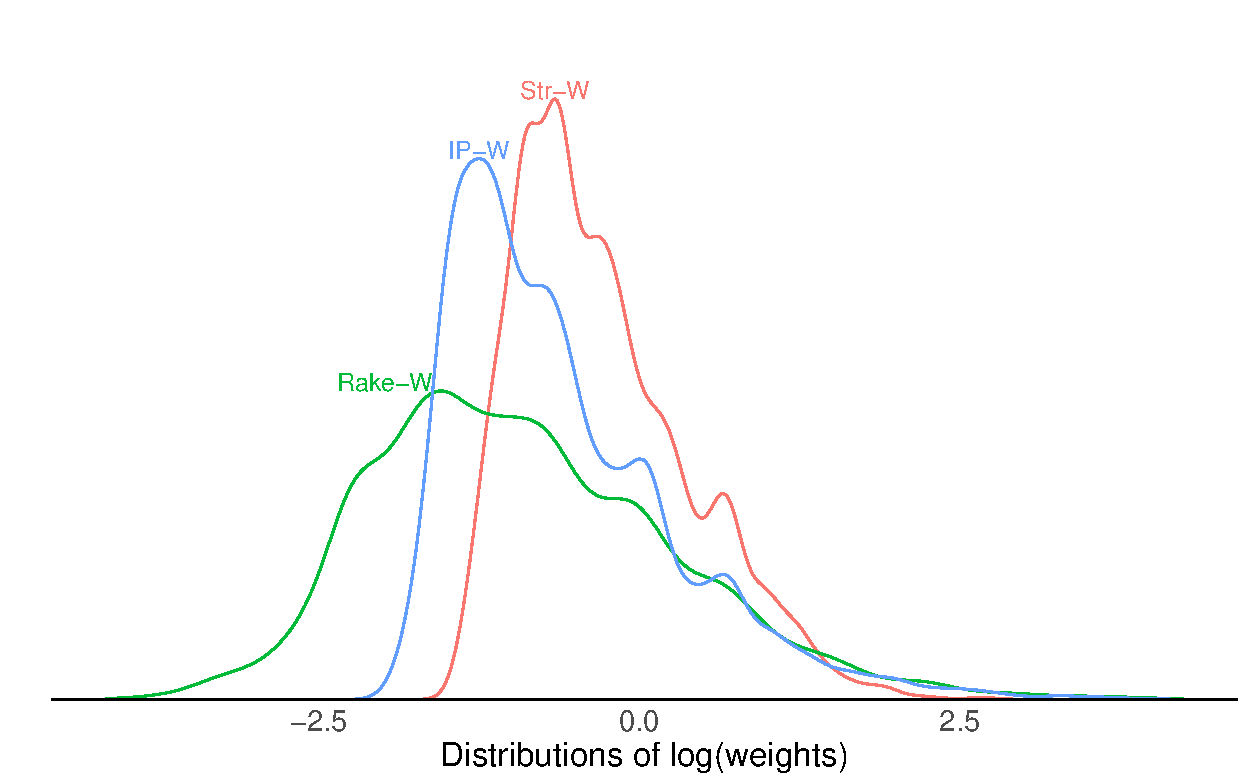
\includegraphics[width=.475\textwidth]{plot/weight-var8-case2.pdf}&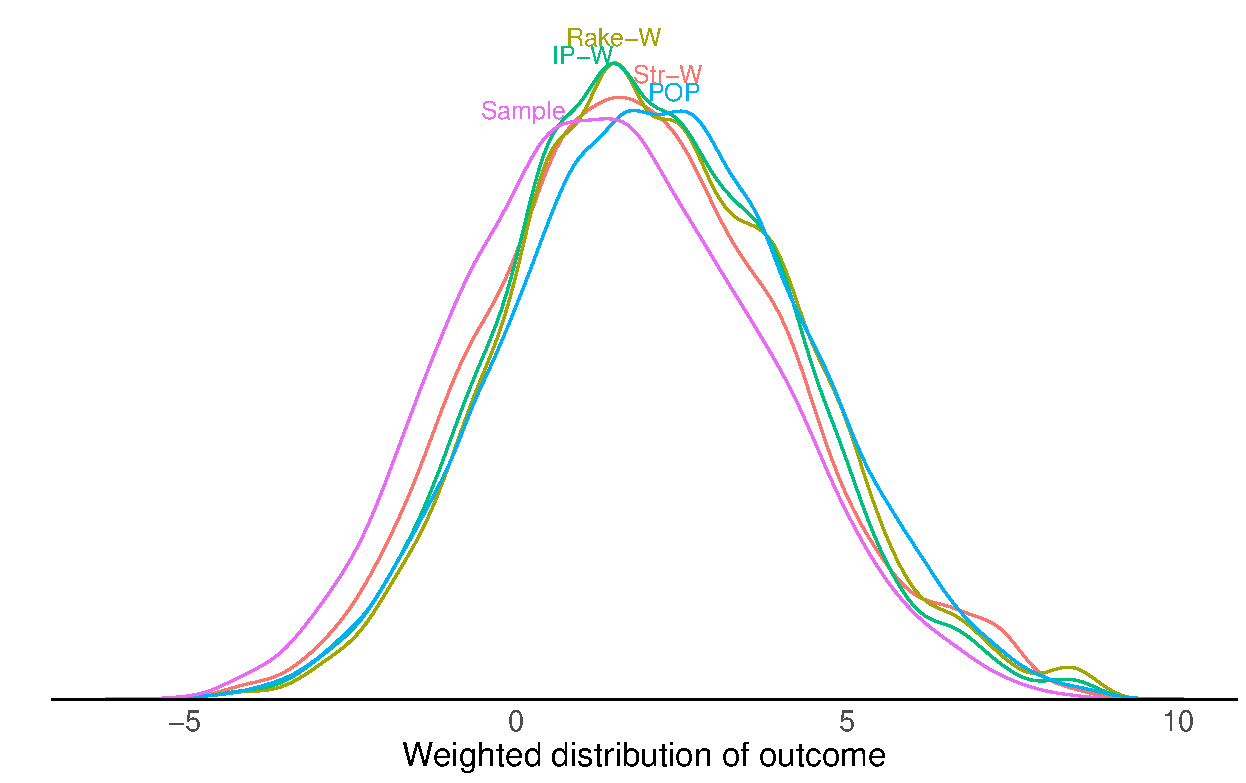
\includegraphics[width=.475\textwidth]{plot/weighted-case2-density.pdf}
\end{tabular}
\caption{\em Comparison of generated weights after logarithm transformation and weighted outcome distributions under a very unbalanced design. Str-W: model-based weighting under structure prior; Rake-W: weighting via raking adjustment; and IP-W: inverse probability of selection weighting. Sample: sample distribution of the outcome; and POP: population distribution of the outcome. The model-based weights are more stable and generate a more smoothed outcome distribution after weighting than the raking weights and the inverse probability of selection weights, }
\label{sim2-weight}
\end{figure} 


We examine the inference for the overall mean and domain means across the marginal levels and for nonwhite young adults. The conclusions are the same as that in Section~\ref{3var}. Model-based prediction outperforms weighting inference with smallest bias and SE. The benefit can be explained by that the model uses the population information for empty cell prediction under regularization. Model-based weighting inference has smaller SEs than that with classical weighting. Even when the selection probabilities depend on only main effects, raking yields small bias but performs badly with large SEs. 

Under the very unbalanced design, the model-based weighting inference under structure prior setting is more efficient than that under independent prior setting or with poststratification weights. We compare the SEs of the marginal mean estimates of the eight weighting variables from the three weighting methods and plot the relative ratios in the left plot of Figure~\ref{sim2-se}. The model-based weighting inference has smaller SEs than the poststratification weighting, while the weighting under structure prior setting has the smallest SEs. Because the sample sizes and the domain sizes are large and the data generation model is sparse, the model-based weighting inference has a little but not much improvement over the poststratification weighting inference due to small smoothing effect. 

The model-based prediction and inference under the structure prior setting are more efficient than that under the independent prior setting. The SEs are smaller with the structure prior than those with the independent prior in the right plot of Figure~\ref{sim2-se}. To  demonstrate the efficiency gain, we look at the SEs for the population cell estimates. The Bayesian structural inference generally has smaller variability than that with independent prior, especially in the sparse scenarios.
  

 \begin{figure}
\centering
\begin{tabular}{cc}
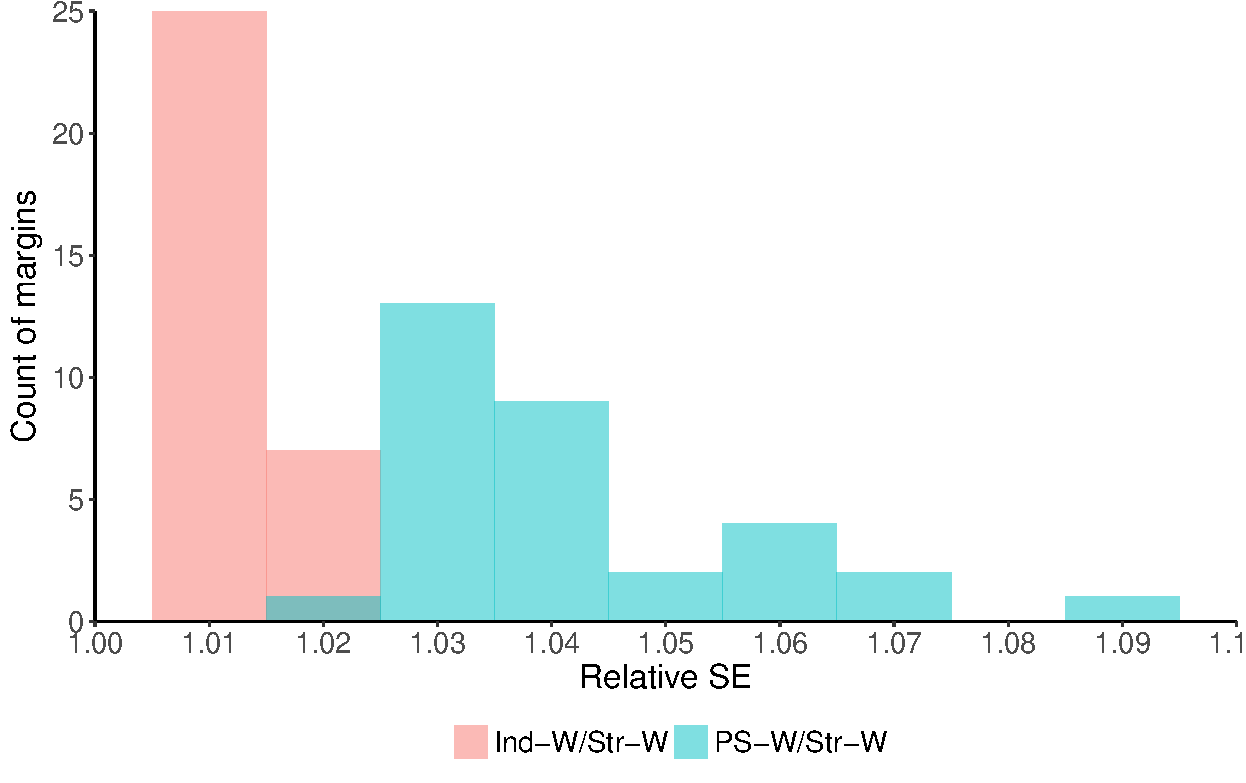
\includegraphics[width=.475\textwidth]{plot/var8_w_se_case2.pdf}&
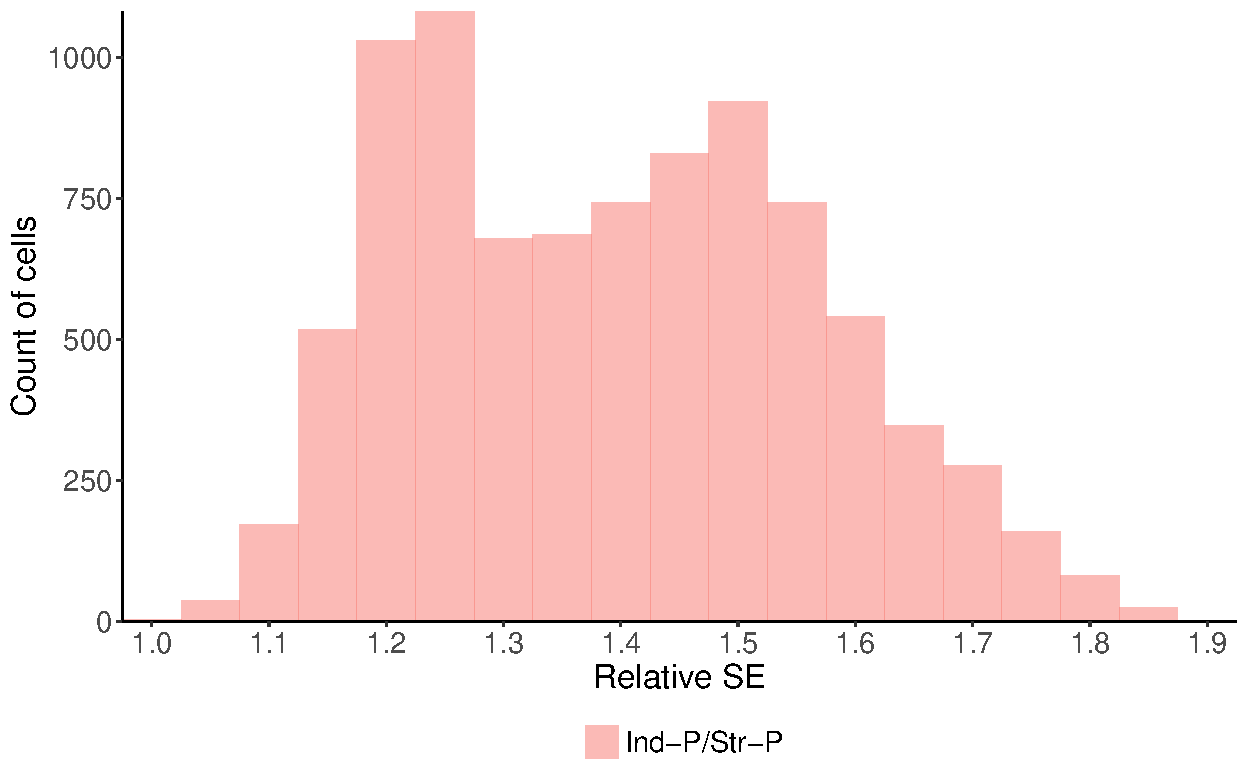
\includegraphics[width=.475\textwidth]{plot/var8_p_se_case2.pdf}\\
\end{tabular}
\caption{\em Efficiency comparison of prediction and weighting performances on finite population domain inference under a very unbalanced design. The left plot examines the mean estimation across the margins defined by the eight weighting variables. The right plots presents the population cell mean estimation. The model-based weighting and prediction under the structure prior distribution yield smaller SEs than those under independent prior. Model-based weighting yields smaller SEs than poststratification weighting.}
\label{sim2-se}
\end{figure} 


We assume different outcome and selection models with different covariates with scenarios summarized in Table~\ref{s2-design} and achieve the same evaluation conclusions. 

%%%%%%%%%%%%%%%%%%%%%%%%%%%%%%%%%%%%%%%%%%%
\section{Application to Longitudinal Study of Wellbeing}
\label{application}

With the background introduced in Section~\ref{problem}, we apply the prediction and weighting inference to the NYC Longitudinal Study of Wellbeing (LSW). We match the LSW to the adult population via Census data from the American Community Survey. We would like to conduct finite population and domain inference and generate weights allowing for general analysis use. The outcome of interest is the self-reported score of life satisfaction on a 1--10 scale.  We model the outcome  as normally distribution, which is not quite correct given that the responses are discrete, but should be fine in practice for the goal of estimating averages. We first include the same eight weighting variables to construct the poststratification cells and use the same estimation model as those in Section~\ref{8var} under the structure prior setting. The posterior inference shows that the variables {\em sex, cldx, eldx}, and {\em psx} are not predictive, and neither are the related high-order interactions. The scale estimates of such terms have posterior median values close to 0 and several large values as long tails. The posterior samples of scales for several high-order interactions among the remaining four variables concentrate around 0, showing these quantities are not predictive. Another complexity is that, for the sample cells of the LSW, the corresponding population cells are not available in the ACS data. This could happen because the sampling framework is not the ACS survey. The population information is unknown for such cells, and untestable assumptions have to be made. The model fitting improves after variable selection when we check the prediction errors for cell estimates.

Hence, we use four weighting variables after selection, {\em age, eth, edu} and {\em pov}, which constructs 500 poststratification cells. The 2002 units in the LSW spread out in 359 cells. The largest sample cell has 86 units, while 92 cells have only one unit. The covariates in the model (\ref{regression}) for cell estimates include the main effects of the four variables, five two-way interactions ({\em age * eth}, {\em age * edu}, {\em eth * edu}, {\em age * inc} and {\em eth * inc}), and two three-way interactions ({\em age * eth * edu} and {\em age * eth * inc}). We implement the fully Bayesian inference with the structure prior distributions. We are interested in estimating the average score of life satisfaction for overall and several subgroups of NYC adults, and construct weights for general analysis purposes using the LSW. 

The posterior median of the unit scale inside cells $\sigma_y$ is 1.77 with 95\% interval $[1.72,1.82]$. The posterior median of the group variance $\sigma_{\theta}^2$ is 0.47 with 95\% interval $[0.23, 1.82]$. These lead to large shrinkage effects between 0.08 and 0.86 with mean 0.64 across cells. The posterior mean values of the model-based weights are presented in the left plot of Figure~\ref{lsw-weight}. We can generate the raking weights after adjustment for the marginal distributions of the four weighting variables and poststratification weights based on the ACS data. The population information is obtained after applying the ACS personal weights.

Comparing with the classical weights, our model-based weights have smaller variability with standard deviation 0.36 and the ratio of the maximum and minimum value 5.0, and these values are much smaller than those for the raking and poststratification weights, as shown in Table~\ref{lsw-est}. The right plot in Figure~\ref{lsw-weight} shows the distribution of the lift satisfaction score after weighting. The model-based weighted distributions and classically weighted distributions are similar as expected, and adjust for the sample distribution by upweighting the high scores and downweighting the low scores. The LSW oversamples poor residents who tend not be satisfied with life, and the weighting adjustment balances the discrepancy.

  %Fig 1:  text on x and y-axes should be larger.  Also the figure needs more the caption:  we need to say what is the point of all this.
%Fig 2:  Remove y-axes and labels entirely.  Also, x-axis should be at y=0 (that is, yaxs="i").  In addition, label the different curves directly (using text(), putting in the locations by hand, an also using colors for these texts) rather than having a legend.
%Fig 3:  Again, text is too small, and, again, x-axis should be at y=0.
%Fig 4:  See comments on figure 2.
%Fig 5:  See comments on figure 1.
%Table 1:  What are Str-P, Str-W, Rake-W, PS-W?

 \begin{figure}
\centering
\begin{tabular}{cc}
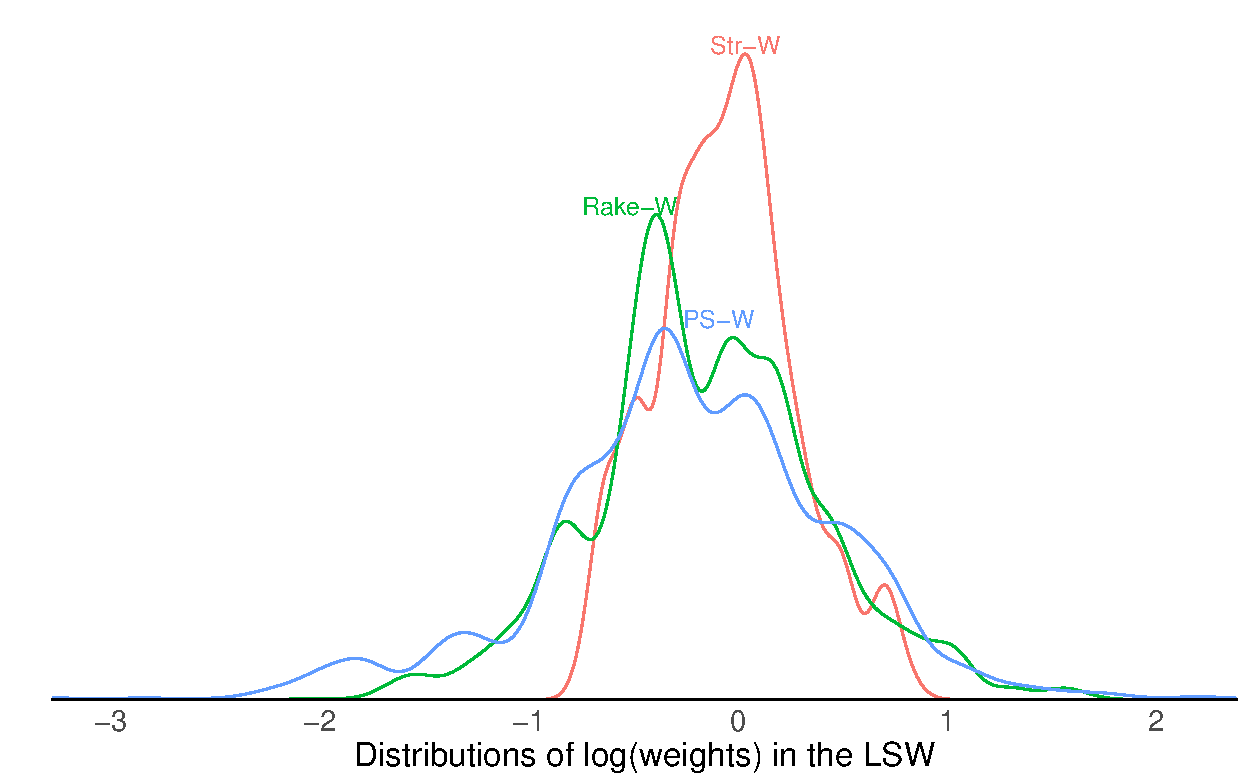
\includegraphics[width=.475\textwidth]{plot/weight-lsw.pdf}&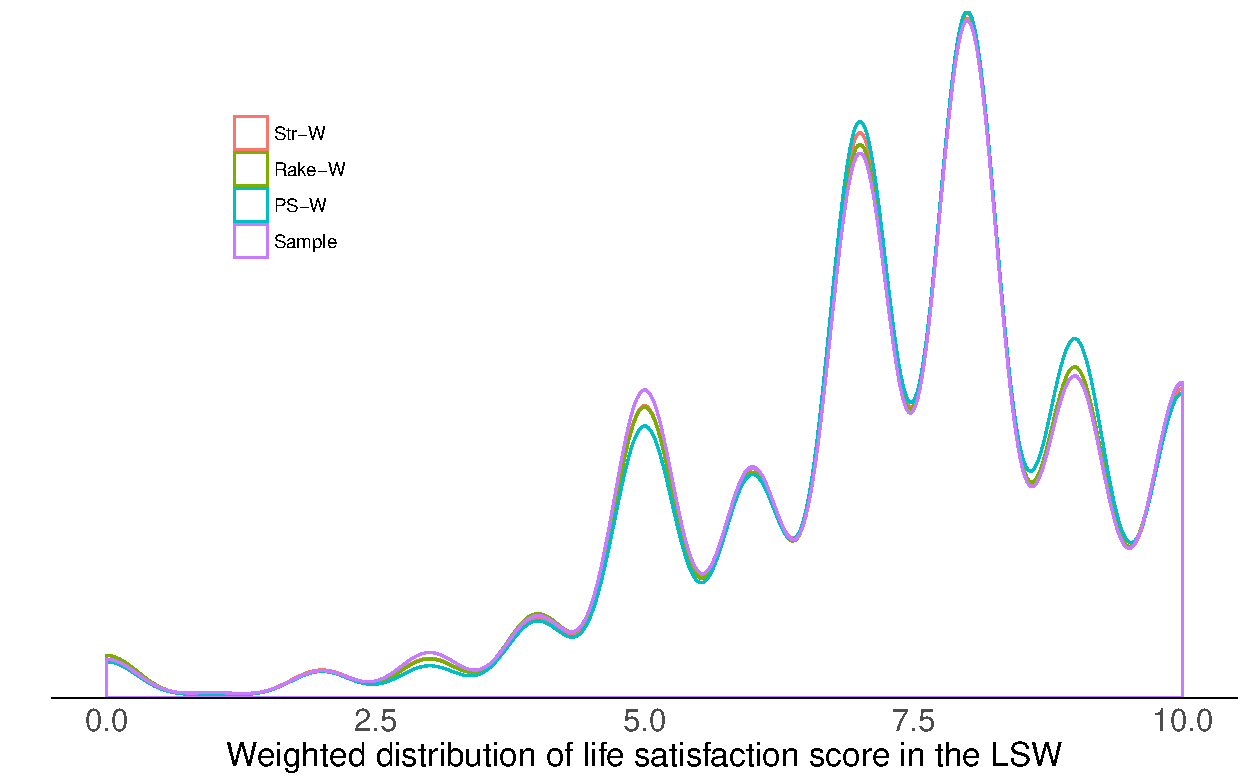
\includegraphics[width=.475\textwidth]{plot/weighted-lsw-density.pdf}
\end{tabular}
\caption{\em Comparison of generated weights after logarithm transformation and weighted distributions of life satisfaction score in the LSW. Str-W: model-based weighting under structured prior; Rake-W: weighting via raking adjustment; IP-W: inverse probability of selection weighting, and Sample: sample distribution of the outcome. The weighted distributions are similar between model-based weights and classical weights, but model-based weights are more stable than classical weights.}
\label{lsw-weight}
\end{figure} 


\begin{table}
\centering
\begin{tabular}{lllll}
& Str-P & Str-W & Rake-W & PS-W \\ 
  \hline
SD of weights / mean of weights & & 0.357 & 0.664 & 0.798 \\ 
Max weight / min weight &  & 5.0 & 81 & 275 \\ 
  \hline
 \multicolumn{5}{l}{Overall average for NYC adults ($n=2002$)}\\
  Est & 7.24 & 7.24 & 7.24 & 7.30 \\ 
  SE & 0.05 & 0.05 & 0.05 & 0.06\\ 
  \hline
 \multicolumn{5}{l}{\begin{tabular}{@{}l@{}}Average for middle-aged, college-educated whites with poverty gap $> 300\%$ ($n=222$)\end{tabular}}\\
Est & 7.57 & 7.34 & 7.34 & 7.34\\ 
SE & 0.11 & 0.11 & 0.11 & 0.11 \\ 
 \hline
\multicolumn{5}{l}{\begin{tabular}{@{}l@{}}Average for elders with poverty gap $> 300\%$ ($n=170$)\end{tabular}}\\
Est & 7.47 & 7.89 & 7.93 & 7.99 \\ 
SE & 0.13 & 0.15 & 0.15 & 0.20 \\ 
\hline
 \multicolumn{5}{l}{\begin{tabular}{@{}l@{}}Averages for blacks with poverty gap $< 50\%$ ($n=57$)\end{tabular}}\\
Est & 7.05 & 7.16 & 7.30 & 7.16 \\ 
SE & 0.18 & 0.26 & 0.28 & 0.29
\end{tabular}
\caption{\em Comparison of prediction and weighting performances on estimating various domain averages for life satisfaction in the LSW. Str-P: model-based prediction under the structured prior; Str-W: model-based weighting under structured prior; Rake-W: weighting via raking adjustment; and PS-W: poststratification weighting. }
\label{lsw-est}
\end{table}


Table~\ref{lsw-est} and Figure~\ref{lsw-mar} present the finite population and domain inference. The average score of life satisfaction for NYC adults is 7.24 with standard error 0.05, predicted by the structural model. The estimate is very slightly higher than that under model-based weighting and raking inferences, but lower than the poststratification weighting inference. However, the difference is not significant. For example, the structural model predicts the average score of life satisfaction for middle-aged, college-educated whites with income more than three times the poverty level as
 7.57 with standard error 0.11, higher than that under weighting inferences. However, the predicted scores for elder with relatively high income (7.47 with SE 0.14) and low-income blacks (7.05 with SE 0.18) are lower than those under weighting inferences. The discrepancy could be explained by the nonrepresentativeness of the LSW and the deep interactions included by the model. The subgroup of individuals who are middle-aged, college-educated whites may be undercovered in the LSW with empty cells, with overcoverage among elderly poor blacks. Weighting the collected samples cannot infer or extrapolate inference on those who are not represented in the survey. Though the differences are not significant, inferences conditioning on the collected samples are not design-consistent, especially for the empty cell estimates. Figure~\ref{lsw-mar} shows the model-based prediction yields higher score for young, highly educated and Hispanic NYC adults, but lower score for those with poverty gap $<50\%$, comparing with the weighted inference.

The standard errors are similar for the overall mean estimation between predictions and various weighting inferences because of the large sample size. For domain estimation, the model-based prediction and weighting are more efficient than that with raking and poststratification weighting, and the model-based prediction has the smallest standard error. The efficiency gains of model-based prediction and weighting are further demonstrated by domain mean estimation for life satisfaction scores across the marginal levels of four weighting variables, shown in Figure~\ref{lsw-mar}. The model-based prediction and weighting particularly improve small domain estimation and increase the efficiency. 

 \begin{figure}
\centering
\begin{tabular}{cc}
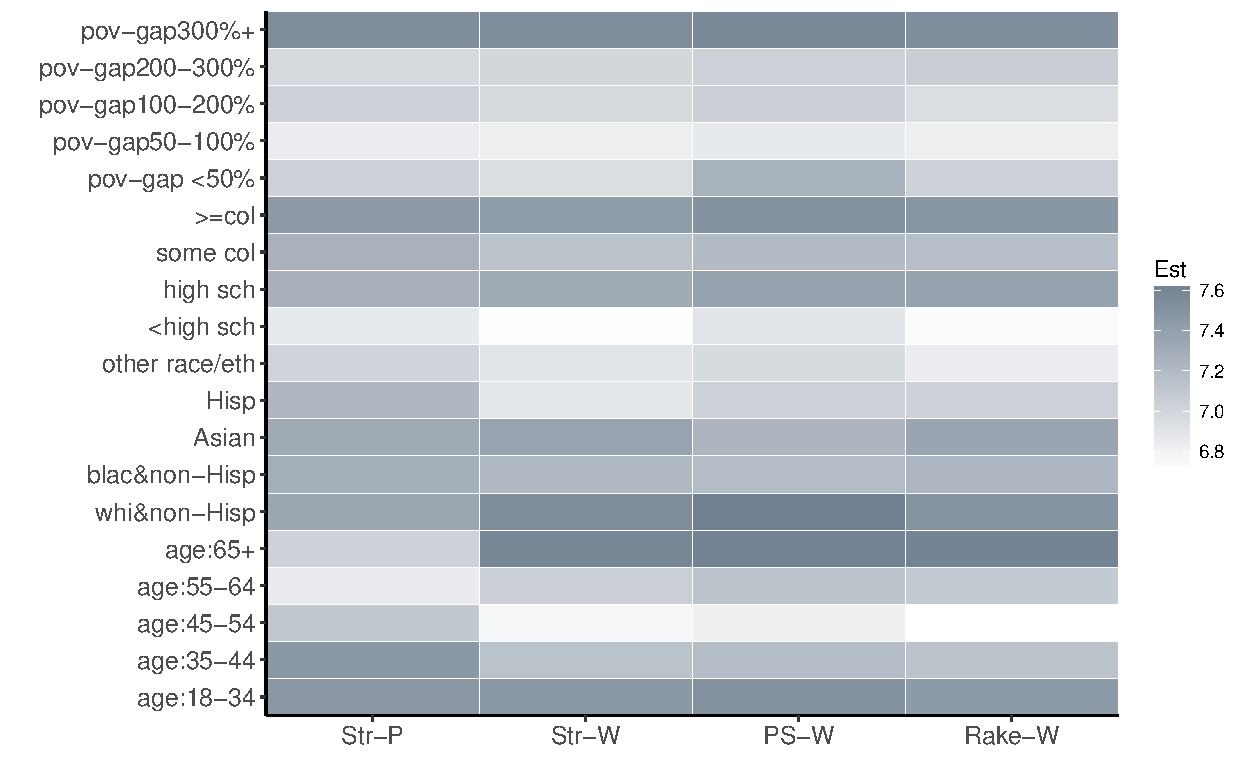
\includegraphics[width=.475\textwidth,height=2.5in]{plot/lsw_mar_est.pdf}&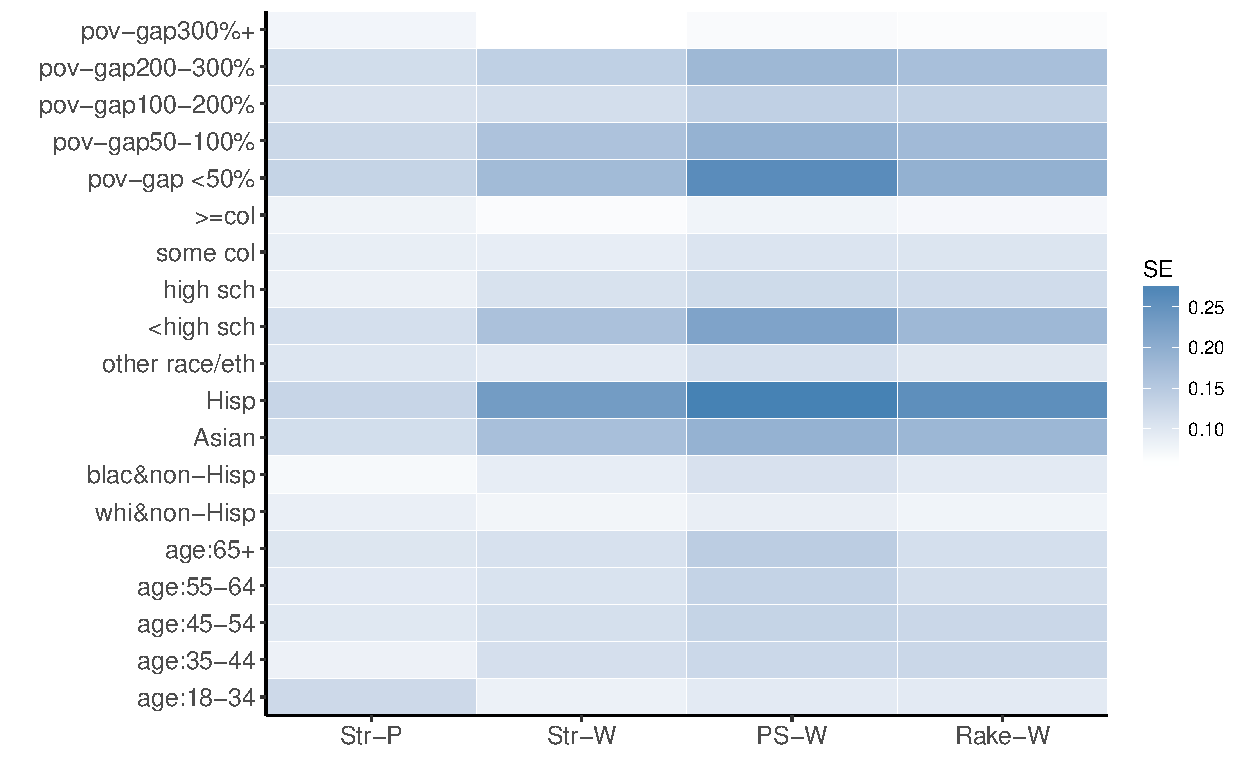
\includegraphics[width=.475\textwidth,height=2.5in]{plot/lsw_mar_se.pdf}
\end{tabular}
\caption{\em Comparison of predictions and weighting performances on estimating life satisfaction score across the margins of four weighting variables in the LSW. Str-P: model-based prediction under the structured prior; Str-W: model-based weighting under structured prior; Rake-W: weighting via raking adjustment; and PS-W: poststratification weighting. Model-based predictions and weighting generate different estimates for several subsets and are generally more efficient comparing with classical weighting.}
\label{lsw-mar}
\end{figure} 


In practice, survey practitioners often compare the weighted distribution of socio-demographics with the population distribution to check the weighting, or for the weighting variables. We calculate the Euclidean distances between the weighted distributions and the population distribution for the main effects and high-order interactions among the four weighting variables in the LSW, shown in Table~\ref{prob-dist} in Appendix~\ref{appendix}. Raking focuses on adjusting for the marginal distributions of weighting variables but distorts the joint distributions. The poststratification weighting adjusts for the joint distribution, but empty cells in the sample present from the exact matching. The model-based weighting smooths the poststratification weightings and outperforms raking to match the distributions of three-way and four-way interaction terms. Practitioners often rely the marginal distributions to evaluate weighting performances, thus in favor of raking. However, raking yields high variable inferences, shown in the Section~\ref{simulation}, even in the cases when raking adjustment is correct. 
Modification of model-based weighting to satisfy such desire will be a future extension.

%%%%%%%%%%%%%%%%%%%%%%%%%%%%%%%%%%%%%%%%%%%%%%%%%
\section{Discussion}
\label{discussion}

We combine Bayesian prediction and weighting as a unified approach to survey inference. Multilevel regression with structured prior distributions and poststratification on the population inference yield efficient and design-consistent estimation. The computation is implemented via Stan, and the software development promotes the model-based approaches in survey research and operational practice. We construct stable model-based weights to solve the problems of classical weights. This article builds up the model-based prediction and weighting framework and serves as the first contribution to evaluate the statistical properties of model-based weights and compare the performances with classical weighting. Model-based weights are smoothed across poststratification cells and improve small domain estimation. 

The structured prior uses the hierarchical structure between main effects and high-order interaction terms to introduce multiplicative constraints on the corresponding scale parameters and informs variable selection after post-processing the posterior inferences. The Bayesian structural model yields more stable inference than that with independent prior distributions. Furthermore, the unified prediction and weighting approach is well equipped to deal with complex survey designs and big data in surveys, such as streaming data and combining multiple survey studies. 

The general MRP framework is open to flexible modeling strategies. In this article, we illustrate by a regression model with all variables of interest and the high-order interactions and incorporate structured prior distributions for regularization. Other approaches, such as nonparametric models and machine learning tools, can be implemented under the MRP framework, being robust against model misspecification. \cite{bnfp:ba15} use Gaussian process regression models to borrow information across poststratification cells based on the distances between the inverse inclusion probability weights. Further extensions include applying such flexible approaches to weight smoothing and deriving the model-based weights. 

The broad application opportunities come with various challenges that need further investigation. The model-based weights are outcome dependent, which improves the efficiency but potentially reduces the robustness. Survey organizers prefer a set of weights than can be used for general analysis purpose, without being sensitive to outcome selection. We can compare different weights constructed by several important outcomes and conduct sensitivity analysis. When the model-based weights give different inference conclusions, we recommend choosing the set of weights that generate the most reasonable results, with scientific reasoning and be consistent with population inference. 

The weighted marginal distributions of the weighting variables are a bit different from the population inferences, as in Section~\ref{application}, which does not meet the usual weighting diagnosis standard of survey organizers. The model-weights tend to match the joint distribution of the weighting variables to that in the population, but weight smoothing may bring in bias. Tradeoff constraints can be induced to the model to match the marginal distributions. 

Another practical challenge is that, the population distribution of the weighting variables may be unknown, that is, the population poststratification cell sizes $N_j$'s are unknown. A supplemental model is needed to allow estimation of this information from the sample. When marginal distributions are available, \cite{rake:little91} discuss an equivalent model approach for raking. Auxiliary variables or additional information on the population can be included in the Bayesian framework. Some auxiliary variables' population distribution may not be available in the census database, such as the number of phones, and we can estimate from other surveys as reference samples.

The model-based predictions and weighting inferences need further extensions to handle non-continuous outcome, inference on regression coefficients and non-probability or informative sampling designs~\citep{Kim:Skinner:BM13}. It will be useful to link these ideas on survey inference with biostatistical and econometric literatures on inverse probability and doubly robust weighting~\citep{kang:schafter07}.

\bibliographystyle{chicago}
\bibliography{mrp-weighting}

\appendix

\section{Stan code}\label{stancode}
Here we present the Stan program {\tt structureweighting\_3var.stan} for our model when three weighting variables and all the high-order interaction terms are included, as in the slightly unbalanced design.
\begin{small}\begin{verbatim}
data {
  int<lower=0> n;//sample size
  int<lower=0> J;//#cells
  int<lower=0> J_true; //#cells in population
  int<lower=0> q;//#variables
  int<lower=0> J_use[J]; //occupied cells
  vector[J] N_cell;
  vector[J_true] N_cell_true;
  vector[J] n_cell;
  vector[J] y_cell; //continuous outcome
  real<lower=0> ss_cell; //sum of variance in cells
  int<lower=0> cell_str[J_true,q]; //variable values allocated to cells
  int<lower=0> J_age; //levels
  int<lower=0> J_eth;
  int<lower=0> J_edu;
  int<lower=0> J_age_eth;
  int<lower=0> J_age_edu;
  int<lower=0> J_eth_edu;
  int<lower=0> J_age_eth_edu;
}
parameters {
  real alpha; //intercept
  vector[J_age] alpha_age;
  vector[J_eth] alpha_eth;
  vector[J_edu] alpha_edu;
  vector[J_age_eth] alpha_age_eth;
  vector[J_age_edu] alpha_age_edu;
  vector[J_eth_edu] alpha_eth_edu;
  vector[J_age_eth_edu] alpha_age_eth_edu;
  real<lower=0> lambda_m[q];
  real<lower=0> sigma_m;
  real<lower=0> lambda_inter[2];
  real<lower=0> sigma_y;
}
transformed parameters{
  vector[J] mu_cell;
  vector[J] sigma_y_cell;
  for (j in 1:J){
    mu_cell[j] = alpha + alpha_age[cell_str[J_use[j],1]] * sigma_m * lambda_m[1] + 
      alpha_eth[cell_str[J_use[j],2]] * sigma_m * lambda_m[2] + 
      alpha_edu[cell_str[J_use[j],3]] * sigma_m * lambda_m[3] +
      alpha_age_eth[(cell_str[J_use[j],2]-1) * J_age + 
      cell_str[J_use[j],1]] * lambda_inter[1] * lambda_m[1] * lambda_m[2] * sigma_m +
      alpha_age_edu[(cell_str[J_use[j],3]-1) * J_age + 
      cell_str[J_use[j],1]] * lambda_inter[1] * lambda_m[1] * lambda_m[3] * sigma_m +
      alpha_eth_edu[(cell_str[J_use[j],3]-1) * J_eth + 
      cell_str[J_use[j],2]] * lambda_inter[1] * lambda_m[2] * lambda_m[3] * sigma_m + 
      alpha_age_eth_edu[(cell_str[J_use[j],3]-1) * J_eth * J_age + 
      (cell_str[J_use[j],2]-1) * J_age + cell_str[J_use[j],1]] * lambda_inter[2] *
      lambda_m[1] * lambda_m[2] * lambda_m[3] * sigma_m;
  }
  for (j in 1:J){
    sigma_y_cell[j] = sigma_y / sqrt(n_cell[j]);
  }
}       
model {
  alpha ~ normal(0,100);
  alpha_age ~ normal(0,1);
  alpha_eth ~ normal(0,1);
  alpha_edu ~ normal(0,1);
  alpha_age_eth ~ normal(0,1);
  alpha_age_edu ~ normal(0,1);
  alpha_eth_edu ~ normal(0,1);
  alpha_age_eth_edu ~ normal(0,1);
  sigma_m ~ normal(0,1); //student_t(3,0,1);
  sigma_y ~ cauchy(0,5);
  lambda_inter ~ normal(0,1);
  lambda_m ~ normal(0,1); //student_t(3,0,1);
  y_cell ~ normal(mu_cell,sigma_y_cell);
  ss_cell / pow(sigma_y,2) ~ chi_square(n-1);
  target += log(2) - 3 * log(sigma_y);
}
generated quantities{
  vector[J] y_cell_new;
  vector[J] w_new;
  vector[J] w_new_ex;
  vector[J] ps_w;
  real pri_var;
  vector[J_true] mu_cell_pred;
  real theta_pred;
  real theta_sample;
  pri_var = square(sigma_m) *
    (square(lambda_m[1]) + square(lambda_m[2]) + square(lambda_m[3]) + 
    square(lambda_inter[1] * lambda_m[1] * lambda_m[2]) +
    square(lambda_inter[1] * lambda_m[1] * lambda_m[3]) +
    square(lambda_inter[1] * lambda_m[2] * lambda_m[3]) +
    square(lambda_inter[2] * lambda_m[1] * lambda_m[2]));
  for (j in 1:J){
    y_cell_new[j] = normal_rng(mu_cell[j],sigma_y_cell[j]);
    //1-ps_w as the shrinkage effect
    ps_w[j] = pow(sigma_y_cell[j],-2)/(pow(sigma_y_cell[j],-2) + 1/pri_var); 
    w_new[j] = ps_w[j] * N_cell[j]/sum(N_cell)/n_cell[j]*n + 1 - ps_w[j];
  }
  for (j in 1:J_true){
    mu_cell_pred[j] = alpha + alpha_age[cell_str[j,1]] * sigma_m * lambda_m[1] + 
      alpha_eth[cell_str[j,2]] * sigma_m * lambda_m[2] + 
      alpha_edu[cell_str[j,3]] * sigma_m * lambda_m[3] +
      alpha_age_eth[(cell_str[j,2]-1) * J_age + 
      cell_str[j,1]] * lambda_inter[1] * lambda_m[1] * lambda_m[2] * sigma_m +
      alpha_age_edu[(cell_str[j,3]-1) * J_age + 
      cell_str[j,1]] * lambda_inter[1] * lambda_m[1] * lambda_m[3] * sigma_m +
      alpha_eth_edu[(cell_str[j,3]-1) * J_eth + 
      cell_str[j,2]] * lambda_inter[1] * lambda_m[2] * lambda_m[3] * sigma_m + 
      alpha_age_eth_edu[(cell_str[j,3]-1) * J_eth * J_age + 
      (cell_str[j,2]-1) * J_age + cell_str[j,1]] * lambda_inter[2] * 
      lambda_m[1] * lambda_m[2] * lambda_m[3] * sigma_m;
  }
 theta_pred = mu_cell_pred' * N_cell_true / sum(N_cell_true);
 theta_sample = mu_cell' * N_cell / sum(N_cell);
}
\end{verbatim}\end{small}

\section{R code}
Here we present the R code for fitting the Stan program in Appendix \ref{stancode}.

\begin{small}\begin{verbatim}
#----------data simulation-----------------#
###ACS data
acs_pop<-read.dta("data/acs_nyc_2011_wpov1.dta",convert.factors = FALSE)
acs_ad <- acs_pop[as.numeric(acs_pop$age)>=18,] 
##age
age_tr<-acs_ad$age #at least 18
acs_ad$age_dc<-age_tr #discretization
acs_ad$age_dc[age_tr<=34]<-1 #18-34
acs_ad$age_dc[age_tr<=44 & age_tr>34]<-2
acs_ad$age_dc[age_tr<=54 & age_tr>44]<-3
acs_ad$age_dc[age_tr<=64 & age_tr>54]<-4
acs_ad$age_dc[age_tr>64]<-5

###race
# race 1 "1 White Non-Hispanic" 2 "2 Black Non-Hispanic" 
#3 "3 Asian" 4 "4 Other" 5 "5 Hispanic"
acs_ad$race_dc<-acs_ad$racex

#educat 4
#recode qi5 (1/2=1) (3/4=2) (5/6=3) (7/8=4) (98/99=.), gen(educat)

q <- 3

J_age <- length(unique(acs_ad$age_dc))
J_eth <- length(unique(acs_ad$race_dc))
J_edu <- length(unique(acs_ad$educat))

N<-dim(acs_ad)[1]

acs_ad$age_dc<-as.factor(acs_ad$age_dc)
acs_ad$race_dc<-as.factor(acs_ad$race_dc)
acs_ad$educat<-as.factor(acs_ad$educat)

options("contrasts")
age<-model.matrix(~age_dc, acs_ad)
race<-model.matrix(~race_dc,acs_ad)
edu<-model.matrix(~educat,acs_ad)

age_race<-model.matrix(~age_dc:race_dc, acs_ad)[,-1]
age_edu<-model.matrix(~age_dc:educat, acs_ad)[,-1]
race_edu<-model.matrix(~race_dc:educat, acs_ad)[,-1]

age_race_edu<-model.matrix(~age_dc:race_dc:educat, acs_ad)[,-1]

###simulate Y
betaY_age<-matrix(seq(0.5, 4,length=dim(age)[2]),dim(age)[2],1)
betaY_race<-matrix(seq(-2, 2,length=dim(race)[2]),dim(race)[2],1)
betaY_edu<-matrix(seq(3, 0,length=dim(edu)[2]),dim(edu)[2],1)

betaY_age_race<-matrix(0,dim(age_race)[2],1)
betaY_age_edu<-matrix(0,dim(age_edu)[2],1)
betaY_race_edu<-matrix(0,dim(race_edu)[2],1)
betaY_age_race_edu<-matrix(0,dim(age_race_edu)[2],1)

muY <- age%*%betaY_age + race %*% betaY_race + edu%*%betaY_edu + 
  age_race%*%betaY_age_race + age_edu%*%betaY_age_edu + race_edu%*%betaY_race_edu + 
  age_race_edu%*%betaY_age_race_edu 
Y<-rnorm(N) + muY

###simuate I

betaI_age<-matrix(seq(-2, -1,length=dim(age)[2]),dim(age)[2],1)
betaI_race<-matrix(seq(-1, 2,length=dim(race)[2]),dim(race)[2],1)
betaI_edu<-matrix(seq(0, 2,length=dim(edu)[2]),dim(edu)[2],1)

betaI_age_race<-matrix(sample(-1:1,dim(age_race)[2],replace=T),dim(age_race)[2],1)
betaI_age_edu<-matrix(sample(-1:1,dim(age_edu)[2],replace=T),dim(age_edu)[2],1)
betaI_race_edu<-matrix(sample(-1:1,dim(race_edu)[2],replace=T),dim(race_edu)[2],1)
betaI_age_race_edu<-matrix(sample(seq(-1,1,by=0.2),dim(age_race_edu)[2],replace=TRUE),
  dim(age_race_edu)[2],1)
sel_prob <- 1/(1+exp(-(-2+age%*%betaI_age + race %*% betaI_race + edu%*%betaI_edu + 
  age_race%*%betaI_age_race + age_edu%*%betaI_age_edu + race_edu%*%betaI_race_edu + 
  age_race_edu%*%betaI_age_race_edu)))
pop_cell_id<-rep(0,N)
cell_str<-matrix(0,J_age*J_eth*J_edu,q)
j<-0
for (i3 in 1:J_edu){
  for (i2 in 1:J_eth){
    for (i1 in 1:J_age){
      j <- (i3-1) * J_eth * J_age + (i2-1) * J_age + i1
      pop_cell_id[acs_ad$age_dc==i1& acs_ad$race_dc==i2 & acs_ad$educat==i3]<-j
      cell_str[j,]<-c(i1,i2,i3)
    }
  }
}
J_true<-J_age*J_eth*J_edu
N_cell_true <- as.numeric(table(pop_cell_id))

pop_data<-data.frame(age=acs_ad$age_dc,eth=acs_ad$race_dc,
	edu=acs_ad$educat,pop_cell_id,Y=Y)

mu_cell_true<-aggregate(.~pop_cell_id,data=pop_data,mean)$Y
###------computation-----###
I<-(runif(N)<=sel_prob)

dat<-data.frame(Y=Y[I],age=acs_ad$age_dc[I],eth=acs_ad$race_dc[I],edu=acs_ad$educat[I])

###cell id
n<-dim(dat)[1]

cell_id<-pop_cell_id[I]

J<-length(unique(cell_id))
J_use<-as.numeric(names(table(cell_id)))
n_cell <- as.numeric(table(cell_id))   

N_cell<-as.numeric(table(pop_cell_id))[as.numeric(names(table(cell_id)))]

mu_cell_use<-mu_cell_true[J_use]

y_cell <- aggregate(.~cell_id,data=dat,mean)$Y
ss_cell<-0
for (j in 1:J){
  ss_cell <- ss_cell+sum((dat$Y[cell_id==J_use[j]]-y_cell[j])^2)
}

stan.data_cell <- list(n=n,q=q, J=J, n_cell=n_cell, y_cell=y_cell, ss_cell=ss_cell,
   cell_str=cell_str, N_cell=N_cell, J_true=J_true, J_use=J_use,
   N_cell_true=N_cell_true, J_age=length(unique(dat$age)),
   J_eth=length(unique(dat$eth)),
   J_edu=length(unique(dat$edu)),
   J_age_eth=length(unique(dat$age)) * length(unique(dat$eth)),
   J_age_edu=length(unique(dat$age)) * length(unique(dat$edu)),
   J_eth_edu=length(unique(dat$eth)) * length(unique(dat$edu)),
   J_age_eth_edu=length(unique(dat$age)) * length(unique(dat$eth)) * length(unique(dat$edu))
)
S.compile_cell_sp <- stan(file="structureweighting_3var.stan", data=stan.data_cell)
\end{verbatim}\end{small}

\section{Simulation designs}
\label{appendix}

Here we present the simulation designs, coefficient values, and comparison on the weighted distributions of socio-demographics as a supplement to Section~\ref{simulation} and Section~\ref{application}.

\begin{table}
\begin{center}
\begin{tabular}{c|cc|cc|cc|cc|cc|cc|cc}
&\multicolumn{2}{|c|}{Case 1}&\multicolumn{2}{|c|}{Case 2}&\multicolumn{2}{|c|}{Case 3}&\multicolumn{2}{|c|}{Case 4}&\multicolumn{2}{|c|}{Case 5}&\multicolumn{2}{|c}{Case 6}&\multicolumn{2}{|c}{Case 7}\\
\hline
&O&S&O&S&O&S&O&S&O&S&O&S&O&S\\
age&$\checkmark$&$\checkmark$&$\checkmark$&$\checkmark$&$\checkmark$&$\checkmark$&$\checkmark$&$\checkmark$&$\checkmark$&$\checkmark$&$\checkmark$&$\checkmark$&$\checkmark$&$\checkmark$\\
eth&$\checkmark$&$\checkmark$&$\checkmark$&$\checkmark$&$\checkmark$&$\checkmark$&$\checkmark$&$\checkmark$&$\checkmark$&\checkmark&&$\checkmark$&&$\checkmark$\\
edu&$\checkmark$&$\checkmark$&$\checkmark$&$\checkmark$&$\checkmark$&&$\checkmark$&$\checkmark$&$\checkmark$&&$\checkmark$&$\checkmark$&$\checkmark$&\\
age*eth&$\checkmark$&&&$\checkmark$&$\checkmark$&$\checkmark$&&&&$\checkmark$&&&&$\checkmark$\\
age*edu&$\checkmark$&&&$\checkmark$&$\checkmark$&&&&&&$\checkmark$&&$\checkmark$&\\
eth*edu&$\checkmark$&&&$\checkmark$&$\checkmark$&&&&&&&&&\\
age*eth*edu&$\checkmark$&&&$\checkmark$&$\checkmark$&&&&&&&&&\\
\end{tabular}
\end{center}
\caption{\em Covariates in the outcome (O) and selection (S) models for slightly unbalanced design.}
\label{s1-design}
\end{table}

\begin{table}
\begin{center}
\footnotesize
\begin{tabular}{c|p{4cm}|l|p{4cm}}
&All & Main effects & Two variables\\
\hline
age&(0.5 1.375 2.25 3.125 4)&(0.5 1.375 2.25 3.125 4)&(0.5 1.375 2.25 3.125 4)\\
eth&(-2 -1 0 1 2)&(2 -1 0 1 2)& $\vec{0}$\\
edu&(3 2 1 0)&(3 2 1 0)&(3 2 1 0)\\
age*eth&(4 2 1 1 3 3 2 1 1 1 2 3 2 2 1 4 4 3 2 3 2 4 1 4 1)& $\vec{0}$& $\vec{0}$\\
age*edu&(-2 -1 2 2 1 -2 2 1 0 -2 1 -2 -1 2 1 -1 -1 2 0 2)& $\vec{0}$&(2 0 -2 -2 1 1 -1 -2 -2 -1 -1 1 0 -1 -1 2 2 1 -1 0 )\\
eth*edu&(1 -2 0 -3 -1 0 -1 -2 0 -1 -3 -3 0 -1 -1 0 0 -1 0 -1)& $\vec{0}$& $\vec{0}$\\
age*eth*edu&(-1 -0.5 0.5 -1 -1 -0.5 -1 0 -1 0 -1 0 1 1 0.5 1 1 -1 -1 0 -1 -0.5 -0.5 -1 1 -1 -0.5 -1 1 0 0.5 0.5 1 0.5 1 1 1 0.5 1 0 0 -0.5 0 1 -1 -1 0 -1 -1 -1 -0.5 -0.5 0 1 -1 0 0 -0.5 1 -0.5 0.5 -1 1 0 1 0 -1 0 -0.5 1 -0.5 -1 -0.5 0 0.5 -0.5 1 0.5 -0.5 0.5 0 1 0 1 0.5 0.5 0.5 0 0 -0.5 1 -1 0 1 1 1 1 -0.5 -1 -1)& $\vec{0}$& $\vec{0}$
\end{tabular}
\end{center}
\caption{\em Assumed regression coefficients in the {\em outcome} model for the simulation using a slightly unbalanced design.}
\label{s1-response-coef}
\end{table}

\begin{table}
\begin{center}
\footnotesize
\begin{tabular}{c|p{4cm}|l|p{4cm}}
&All&Main effects & Two variables\\
\hline
Intercept&-2&-2&-2\\
age&(-2 -1.75 -1.5 -1.25 -1)&(0 0.5 1 1.5 2)&(-2 -1.5 -1 -0.5 0)\\
eth&(-1 -0.25 0.5 1.25 2)&(-2 -1.5 -1 -0.5 0)&(-1 -0.5 0 0.5 1)\\
edu&(0 0.67 1.33 2)&(0 1 2 3)& $\vec{0}$\\
age$\times$eth&(1 1 -1 1 -1 1 -1 0 0 -1 0 0 -1 1 0 0 -1 1 1 -1 -1 0 1 -1 1)& $\vec{0}$&(-1 1 1 1 -1 -1 -1 0 -1 -1 -1 -1 1 -1 -1 0 1 1 -1 1 -1 -1 1 0 0)\\
age$\times$edu&(0 1 -1 -1 0 1 1 0 1 0 1 -1 -1 1 1 -1 0 -1 1 1 )& $\vec{0}$& $\vec{0}$\\
eth$\times$edu&(-1 -1 0 -1 -1 1 1 1 1 0 -1 0 -1 0 -1 1 0 -1 -1 -1 )& $\vec{0}$& $\vec{0}$\\
age$\times$eth$\times$edu& (0.8 -0.4 0.6 -0.2 0.8 0.2 0.4 0.8 0.4 -0.6 -0.8 -0.4 -0.8 -0.4 0.4 -1 0.6 -0.8 -0.6 0.6 -0.2 0.2 0.6 -0.6 0 0 -1 -0.2 0.6 0.8 -0.4 0.2 -0.8 0.4 0.6 -0.6 0.8 0 0.2 -1 1 0.4 0 0.8 -0.2 0 0 0.6 -0.8 -0.8 -0.2 0.4 -1 -0.8 1 -0.2 0 0.8 0.6 0.8 -0.2 -0.2 -0.8 1 0.8 0.8 -0.4 -0.8 0.4 -0.4 1 -0.6 -1 -0.6 -0.2 1 1 -0.2 1 0.6 0.4 0.8 0.2 -0.2 -0.6 0 0.8 -0.4 0.4 0.4 0.6 -1 -0.8 -0.8 1 1 0.4 0.6 0.4 0.8)&$\vec{0}$& $\vec{0}$
\end{tabular}
\end{center}
\caption{\em Assumed regression coefficients in the {\em selection}  model for the simulation using a slightly unbalanced design.}
\label{s1-selection-coef}
\end{table}



\begin{table}
\begin{center}
\begin{tabular}{c|cc|cc|cc|cc}
&\multicolumn{2}{|c|}{Case 1}&\multicolumn{2}{|c|}{Case 2}&\multicolumn{2}{|c|}{Case 3}&\multicolumn{2}{c}{Case 4}\\
\hline
&O&S&O&S&O&S&O&S\\
age&$\checkmark$&$\checkmark$&$\checkmark$&$\checkmark$&$\checkmark$&$\checkmark$&$\checkmark$&$\checkmark$\\
eth&$\checkmark$&$\checkmark$&$\checkmark$&$\checkmark$&$\checkmark$&$\checkmark$&$\checkmark$&$\checkmark$\\
edu&$\checkmark$&$\checkmark$&$\checkmark$&$\checkmark$&$\checkmark$&$\checkmark$&$\checkmark$&$\checkmark$\\
sex&$\checkmark$&$\checkmark$&$\checkmark$&$\checkmark$&$\checkmark$&$\checkmark$&$\checkmark$&$\checkmark$\\
pov&$\checkmark$&$\checkmark$&$\checkmark$&$\checkmark$&$\checkmark$&$\checkmark$&$\checkmark$&$\checkmark$\\
cld&&$\checkmark$&&$\checkmark$&&$\checkmark$&$\checkmark$&$\checkmark$\\
eld&$\checkmark$&$\checkmark$&&$\checkmark$&$\checkmark$&$\checkmark$&$\checkmark$&$\checkmark$\\
fam&$\checkmark$&$\checkmark$&&$\checkmark$&$\checkmark$&$\checkmark$&$\checkmark$&$\checkmark$\\
age*eth&$\checkmark$&$\checkmark$&&&$\checkmark$&&&$\checkmark$\\
age*edu&$\checkmark$&$\checkmark$&&&$\checkmark$&&&$\checkmark$\\
eth*edu&$\checkmark$&$\checkmark$&&&$\checkmark$&& &$\checkmark$\\
eth*pov&$\checkmark$&$\checkmark$&&&$\checkmark$&&&$\checkmark$\\
age*pov&$\checkmark$&$\checkmark$&&&$\checkmark$&&&$\checkmark$\\
pov*fam&$\checkmark$&$\checkmark$&&&$\checkmark$&&&$\checkmark$\\
pov*eld&$\checkmark$&$\checkmark$&&&$\checkmark$&&&$\checkmark$\\
pov*cld&&$\checkmark$&&&&&&$\checkmark$\\
age*eth*edu&$\checkmark$&$\checkmark$&&&$\checkmark$&&&$\checkmark$\\
age*eth*pov&$\checkmark$&$\checkmark$&&&$\checkmark$&&&$\checkmark$
\end{tabular}
\end{center}
\caption{\em Covariates in the outcome (O) and selection (S) models for a very unbalanced design.}
\label{s2-design}
\end{table}


\begin{table}
\begin{center}
\footnotesize
\begin{tabular}{c|p{7cm}|p{7cm}}
&O&S\\
\hline
age&(2 0 -2 -2 1)&(0 0.75 1.5 2.25 3)\\
eth&(1 -1 -2 -2 -1)&(-1 -0.5 0 0.5 1)\\
edu&(-1 1 0 -1)&(0 0.67 1.33 2)\\
sex&(-1 2)&(-1 0)\\
pov&(2 1 -1 0 -1)&(0 1 2 3 4)\\
cld&$\vec{0}$&(-1 -0.33 0.33 1)\\
eld&$\vec{0}$&(-2 -1 0)\\
fam&$\vec{0}$&(-1 -0.67 -0.33 0)
\end{tabular}
\end{center}
\caption{\em Assumed regression coefficient values for the outcome (O) and selection (S) models for a very unbalanced design.}
\label{s2-design-case2}
\end{table}



\begin{table}[ht]
\centering
\begin{tabular}{lrrr}
 & Str-W & PS-W & Rake-W \\ 
 \hline
 {\em age} & 0.033 & 0.021 & 0.000\\
 {\em eth}& 0.081 & 0.064 & 0.000 \\ 
{\em edu}  & 0.079 & 0.035 & 0.000 \\ 
{\em inc}& 0.021 & 0.022 & 0.000 \\ 

{\em age * eth}& 0.043 & 0.031 & 0.046 \\
{\em age * edu}& 0.043 & 0.021 & 0.046 \\
{\em age * inc}& 0.023 & 0.015 & 0.029 \\

{\em eth * edu} & 0.056 & 0.042 & 0.049 \\ 
{\em eth * inc}& 0.043 & 0.035 & 0.033 \\ 
{\em edu * inc} & 0.057 & 0.027 & 0.037 \\

{\em age * eth * edu}& 0.032 & 0.022 & 0.050 \\ 
{\em age * eth * inc}& 0.025 & 0.018 & 0.041 \\


{\em age * edu * inc } & 0.031 & 0.015 & 0.036 \\
{\em eth * edu * inc}&0.038 & 0.024 & 0.040 \\
{\em age * eth * edu * inc}& 0.022 & 0.013 & 0.040
\end{tabular}
\caption{\em Euclidean distances between the weighted distributions and the population distribution.}
\label{prob-dist}
\end{table}

\end{document}

